% Based on templates:
%  - http://www.maths.lth.se/matematiklth/exjobb/exjobbarresurs/index.html
%  - https://bitbucket.org/flavius_gruian/msccls/

% Uncomment to use official LTH thesis template
\def\UseCSLTH{true}

% needed to pass table option to xcolor import in cslthse-msc template
\PassOptionsToPackage{table}{xcolor}

\ifx\UseCSLTH\undefined
    \documentclass[a4paper]{article}
\else
    \documentclass[nofilelist]{cslthse-msc}
\fi

% Import common packages that are used in all documents, used in figures
\usepackage[smartEllipses]{markdown}  % For markdown
\def\markdownOptionOutputDir{build}  % Needed, see https://github.com/Witiko/markdown/issues/6#issuecomment-328699108

\usepackage{array}
\usepackage{hyperref}
\usepackage{makecell}
\usepackage{comment}
\usepackage{xargs}
\usepackage{verbatim}
\usepackage{subfig}
\usepackage{booktabs}
\usepackage{changepage}
\usepackage{rotating, graphicx}
\usepackage{multirow}
\usepackage{pdflscape}
\usepackage{afterpage}
\usepackage[export]{adjustbox}
\usepackage[dvipsnames]{xcolor}
\usepackage[bottom]{footmisc}
\usepackage[colorinlistoftodos, prependcaption, textsize=tiny]{todonotes}

% References
\usepackage[backend=biber, style=numeric, sorting=none]{biblatex}
\usepackage{cleveref}

% Formatting
\setlength{\parindent}{0pt}
\setlength{\parskip}{1em}

% Encoding and languages
\usepackage[utf8]{inputenc}
\usepackage[english]{babel}
\usepackage[T1]{fontenc}        % För svenska bokstäver
%\usepackage[swedish]{babel}    %Svenska skrivregler och rubriker

% Graphics
\usepackage{epsfig}
%\usepackage[dvips]{graphics}

% For adding source captions to figures.
% From: https://tex.stackexchange.com/a/246285/36302
\newcommand{\source}[1]{\vspace{-0.3cm} \caption*{\footnotesize{Source: \textit{{#1}}}}}


% Formatting
\setlength{\parindent}{0pt}
\setlength{\parskip}{1em}

% Give penalty for widows and orphans: https://en.wikipedia.org/wiki/Widows_and_orphans
% Should prevents sections to start near the end of a page, but doesn't seem to have much effect.
%\clubpenalty10000
%\widowpenalty10000

% This seems to do what the above was supposed to.
% But it's a bit too aggressive, so maybe disable?
\widowpenalties=3 10000 10000 150

% ignore badness warnings (not working?)
%\vbadness=10000
%\hbadness=10000

% Add subsubsubsection
% As per https://tex.stackexchange.com/a/60212/36302
\usepackage{titlesec}
\setcounter{secnumdepth}{4}
\titleformat{\paragraph}
{\normalfont\normalsize\bfseries}{\theparagraph}{1em}{}
\titlespacing*{\paragraph}
{0pt}{3.25ex plus 1ex minus .2ex}{1.5ex plus .2ex}

% Better formating for values and units
% From https://tex.stackexchange.com/questions/79141/is-there-a-designated-symbol-for-the-negative-sign-in-say-16
\DeclareUnicodeCharacter{2212}{\textminus}% requires a unicode capable editor
\usepackage{siunitx}
\sisetup{
   detect-mode,
   detect-family,
   detect-inline-family=math,
}

% Ensures floats stay in their section
\usepackage[section]{placeins}

\usepackage[english]{datetime2}
\DTMnewdatestyle{dashdate}{%
  \renewcommand{\DTMdisplaydate}[4]{\number##1-\DTMenglishshortmonthname{##2}-\number##3}%
  \renewcommand{\DTMDisplaydate}{\DTMdisplaydate}%
}
\DTMsetdatestyle{iso}

% From: https://tex.stackexchange.com/a/178806/36302
\newcommandx{\add}[2][1=]{\todo[linecolor=red, backgroundcolor=red!25, bordercolor=red, inline, #1]{\textbf{Add:} #2}}
\newcommandx{\unsure}[2][1=]{\todo[linecolor=red, backgroundcolor=red!25, bordercolor=red, #1]{\textbf{Unsure:} #2}}
\newcommandx{\change}[2][1=]{\todo[linecolor=blue, backgroundcolor=blue!25, bordercolor=blue, #1]{\textbf{Change:} #2}}
\newcommandx{\info}[2][1=]{\todo[linecolor=OliveGreen, backgroundcolor=OliveGreen!25, bordercolor=OliveGreen, #1]{\textbf{Info:} #2}}
\newcommandx{\improvement}[2][1=]{\todo[linecolor=Plum, backgroundcolor=Plum!25,bordercolor=Plum, #1]{\textbf{Improve:} #2}}
\newcommandx{\thiswillnotshow}[2][1=]{\todo[disable, #1]{#2}}

\newcommand\myshade{85}
\colorlet{mylinkcolor}{violet}
\colorlet{mycitecolor}{YellowOrange}
\colorlet{myurlcolor}{Aquamarine}

\hypersetup{%
  linkcolor =.,
  citecolor = mycitecolor!\myshade!black,
  urlcolor  = myurlcolor!\myshade!black,
  colorlinks = true,
}

% wide page for side by side figures, tables, etc
\newlength{\offsetpage}
\setlength{\offsetpage}{1.0cm}
\newenvironment{widepage}{\begin{adjustwidth}{-\offsetpage}{-\offsetpage}%
    \addtolength{\textwidth}{2\offsetpage}}%
{\end{adjustwidth}}

% References
\bibliography{zotero}
\bibliography{misc}


% Import title, author, etc.
\def\mytitleen{Classifying brain activity using electroencephalography and automated time tracking of computer use}
\def\mytitlesv{Klassificering av hjärnaktivitet med elektroencephalografi och automatiserad tidsspårning av datoranvändning}

\def\myauthor{Erik Bjäreholt}
\def\myorcid{0000-0003-1350-9677}
\def\myemail{erik@bjareho.lt}


\ifx\UseCSLTH\undefined
    \title{%
        \small DRAFT \today \\
        \small The latest version is available at \href{https://erik.bjareholt.com/thesis/thesis.pdf}{erik.bjareholt.com/thesis/thesis.pdf}\\
        \large --- \\
        \large \par M.Sc. Thesis\\
        \huge \mytitleen\\
    }
    \author{\myauthor\ \orcid{\myorcid} \\(\myemail)}
    \date{\today}
\else
    \title{\mytitleen}
    \svensktitel{\mytitlesv}
    % TODO: Add a subtitle?
    %\subtitle{Discerning reading code vs prose and other device activities, using consumer EEG devices and the open source automated time tracker ActivityWatch}

    \date{\today}
    %\date{January 16, 2015}

    \student{\myauthor}{\myemail}

    \company{RISE}
    \supervisor{Markus Borg, \texttt{markus.borg@\{\href{mailto:markus.borg@cs.lth.se}{cs.lth.se}, \href{mailto:markus.borg@ri.se}{ri.se}\}}}
    \examiner{Elizabeth Bjarnarson, \href{mailto:elizabeth.bjarnason@cs.lth.se}{\texttt{elizabeth.bjarnason@cs.lth.se}}}

    %\geometry{showframe}

    \thesisnumber{LU-CS-EX: 2023-79} % Magic Number! Do not change unless Birger Swahn asks you to do so!
    % default is Master. Uncomment the following for "kandidatarbete"/Bachelor's thesis
    %\thesistype{Bachelor}{Kandidatarbete}

    %\onelinetitle
    %\twolinestitle
    %\threelinestitle
    \fourlinestitle

    \theabstract{We investigate the ability of EEG to distinguish between different activities users engage in on their devices, building on previous research which showed a considerable difference in brain activity between code- and prose-comprehension, as well as differences during the synthesis. We explore multiple classification approaches, including using bandpass features, Riemannian geometry, and deep learning.

We also use the automated time tracker ActivityWatch to track what device activities the user is engaging in. This lets us label EEG data with naturalistic device activity, which we then use to train classifiers of device activity.

Code and a sample dataset is available at \href{https://github.com/ErikBjare/thesis}{github.com/ErikBjare/thesis}.
}

    \acknowledgements{\begin{itemize}
 \item My advisor Markus Borg~\orcid{0000-0001-7879-4371}.
 \item My brother Johan Bjäreholt, for working with me on ActivityWatch all these years.
 \item The NeuroTechX crowd, specifically Morgan Hough~\orcid{0000-0001-5256-413X} and John Griffiths, for their support and time spent helping me.
 \item The people at the LTH Department for Automatic Control, for providing early guidance.
 \item Andrew Jay Keller at Neurosity, for giving me a refurbished Notion DK1 to work with.
 \item Alex K. Chen, for referring me to all the right people.
 \item All the test subjects.
 \item Everyone who's contributed to the open source tools I've used.
\end{itemize}
}

    \keywords{electroencephalography, brain computer interfaces, time tracking, code comprehension, productivity, MSc}
\fi

\makeglossaries
\newglossaryentry{latex}{
    name=latex,
    description={Is a markup language specially suited for 
scientific documents}
}

\newacronym{eeg}{EEG}{Electroencephalography}
\newacronym{fmri}{fMRI}{Functional Magnetic Resonance Imaging}

\newacronym{bac}{BAC}{Balanced Accuracy}
\newacronym{loro}{LORO}{Leave-One-Run-Out}


\begin{document}


\makefrontmatter

% CS template inserts ToC as part of frontmatter
\ifx\UseCSLTH\undefined
    \tableofcontents
\fi

% Pagebreak after ToC
\vfill
\pagebreak

% Don't show notes & TODOs in final version
%\listoftodos[Notes \& TODOs]
%\vfill

\begin{refsection}

\section*{Preface}

When I started university in 2013, I already knew that one day I wanted to work with brain-computer interfaces. During high school I had been soaked in transhumanist and hacker culture, spending more time online than in school.

I had come to the realization that the field was bound to fundamentally change how we interact both with computers and each other. However, I was aware that the field was in its earlier phases, and the work that needed to be done was outside of my expertise at the time.

So I asked how can I set myself up to be in a position to contribute to this impactful field of research. My answer at the time was to learn about data collection and analysis generally, and a couple years later applied my skills building ActivityWatch, as I figured the best approximation about what goes on in my head is what I'm looking at on my computer screen.

What I thought would be a small learning project soon took on a life of its own. People online started showing interest, and soon my brother joined in development. What started as a fun project to analyze my own device usage soon became a popular open source application with thousands of users. At some point it became apparent that once my Master's thesis was to be written, it would involve ActivityWatch one way or another.

As I was finishing up my final exams, I found an old paper in a moving box, it was a thesis proposal I had picked up at a career fair many years back. The proposal was from my advisor Markus Borg, and curious as I was, I contacted him and asked if it was still available. Markus enthusiastically replied, and helped my adapt his suggestion to join it with my previous work on ActivityWatch.

As my thesis work progressed, I learned a lot about brain imaging and BCIs in general, and EEG in particular.

This thesis work has served as my first proper contribution to the field, all according to the plan I had made at the start of my university degree.

The Oxford English Dictionary defines `thesis' as ``a long essay or dissertation involving \emph{personal research}, written by a candidate for a university degree''. I can't think of more ``personal research'' than research in quantified self with personal data.

%\pagebreak

\chapter{Introduction}

% How to write an introduction: https://student.unsw.edu.au/introductions

% Move 1 establish your territory (say what the topic is about)

We live in an age of massive data collection about all manner of things. Whether the goal is scientific, financial, or personal, the rise of computing over the last half century has led to ever increasing data collection and analysis in pursuit of these goals. Yet for some domains, like what goes on inside our heads, we have limited capability for data collection.

Communities like the Quantified Self movement have risen to the challenge of collecting and analyzing highly personal data for insights into our lives and health. But while some data is easily observed, such as steps taken, physical location, and which app one is using, it's more difficult to collect data about ones internal state (like mood, productivity, what one is thinking about), often requiring manual data collection, or approximations constructed from other data.

% other formulation of goals: profits, productivity, sustainability

% Move 2 establish a niche (show why there needs to be further research on your topic)

While within the reach of medical professionals with access to expensive equipment like MRI scanners and high-density EEG setups, the ability for the average individual to collect data about their own brain activity has been limited. However, in recent years the cost of consumer EEG devices has fallen sharply, offering a feasible solution to monitor brain activity during everyday tasks.

% Brain Computer Interfaces (BCIs) have become available as consumer goods, thanks to the economic viability of brain imaging techniques like electroencephalography (EEG). These devices promise to measure different aspects of your mental state: wether you're grasping an object, or how calm you are during your meditation session. Low-cost brain imaging technologies like EEG are therefore suitable as candidates for richer collection about the user's mental state.

% Move 3 introduce the current research (make hypotheses; state the research questions)

In this thesis, we've developed a framework for studying brain activity during various naturalistic device activities. We do so by collecting brain activity data using consumer-grade EEG devices while simultaneously tracking the device activity they're engaging in. We then use that data to train classifiers of device activity.

We also apply similar methodology to a controlled experiment where we try to train a classifier to distinguish between the subject reading code vs prose.

%\section{Background}

People spend more time than ever using computing devices. Work, entertainment, and services, have been steadily moving online over the last few decades and this trend is expected to continue.
While several studies have been tracking how people spend time on their devices, a wider study of how people's app usage is changing over time, and how it varies with demographics, is not publicly available.

Furthermore, how different device activities affect the user behaviorally and neurologically is of interest for many areas of research, including:

\begin{itemize}
    \item psychological well-being, such as depression and social anxiety~\cite{selfhout_different_2009}\cite{shah_nonrecursive_2002}, stress~\cite{mark_stress_2014}, self-esteem, life satisfaction, loneliness, and depression~\cite{huang_time_2017}.
    \item the impact of screen time on children and adolescents~\cite{subrahmanyam_impact_2001}.
    \item attention span among media multitasking adults~\cite{mark_stress_2014}.
    \item enhancing personal productivity~\cite{kim_timeaware_2016}.
\end{itemize}

Understanding device use and the underlying cognitive processes are essential when designing for motivation, engagement and wellbeing in digital experiences~\cite{peters_designing_2018}.

%\add[inline]{Add connection to software developers}

This becomes especially relevant for knowledge workers, in particular software developers, who spend the vast majority of their time working on computers.

Brain imaging techniques such as EEG show a potential to shed light on many of these research questions, and the relationship between device usage and brain activity seems an largely unexplored area worth investigating.

\add[inline]{Mention of Quantified Self movement, and the applicability/usefulness of EEG data to the cause}

\subsection{Automated time trackers}

    Automated time-trackers have been developed for computing devices, with various applications such as tracking hours worked, personal productivity, managing excessive use of social networking sites (SNSs), and studying human behavior.

    \subsubsection{Commercial use}

        Companies like RescueTime~\cite{noauthor_rescuetime_nodate}, Hubstaff~\cite{noauthor_hubstaff_nodate}, and others offer automated time tracking as a service. These services let the user track their screen time by installing a program on their device which tracks the active application and sends the data to their servers for storage and analysis. The user can then view their data in a dashboard on the service's website. Some of these services, like RescueTime and Hubstaff, are marketed towards teams and professionals, who want to keep track of individual and team productivity.

        However, these services have some issues for use by researchers and individuals alike. Notably, their collection of detailed and non-anonymized behavioral data into a centralized system bring significant privacy concerns, especially in cases where the data is shared with a team or an employer.

        Other limitations of these services, such as low temporal resolution and limited event detail, cause additional issues for certain tasks that are timing-sensitive (such as ERPs), or preprocessing steps that can take advantage of high level of detail (like classifying activity).

    \subsubsection{Research use}

        Previous research has been published which used automated time trackers, such as TimeAware~\cite{kim_timeaware_2016} and ScreenLife~\cite{rooksby_personal_2016}. However, these previous contributions are --- like the commercial services --- not open source nor permissively licensed, and therefore not available for external research use nor further development.

    \subsubsection{ActivityWatch}

        The free and open source automated time tracker ActivityWatch~\cite{bjareholt_activitywatch_2020}, previously developed by the author of this thesis together with contributors, addresses aforementioned issues with other software around source availability/licensing, privacy, temporal resolution, event detail, and cross-platform support.

        \todo[inline]{Update screenshot to v0.11}

        \begin{figure}[h]
        \centering
        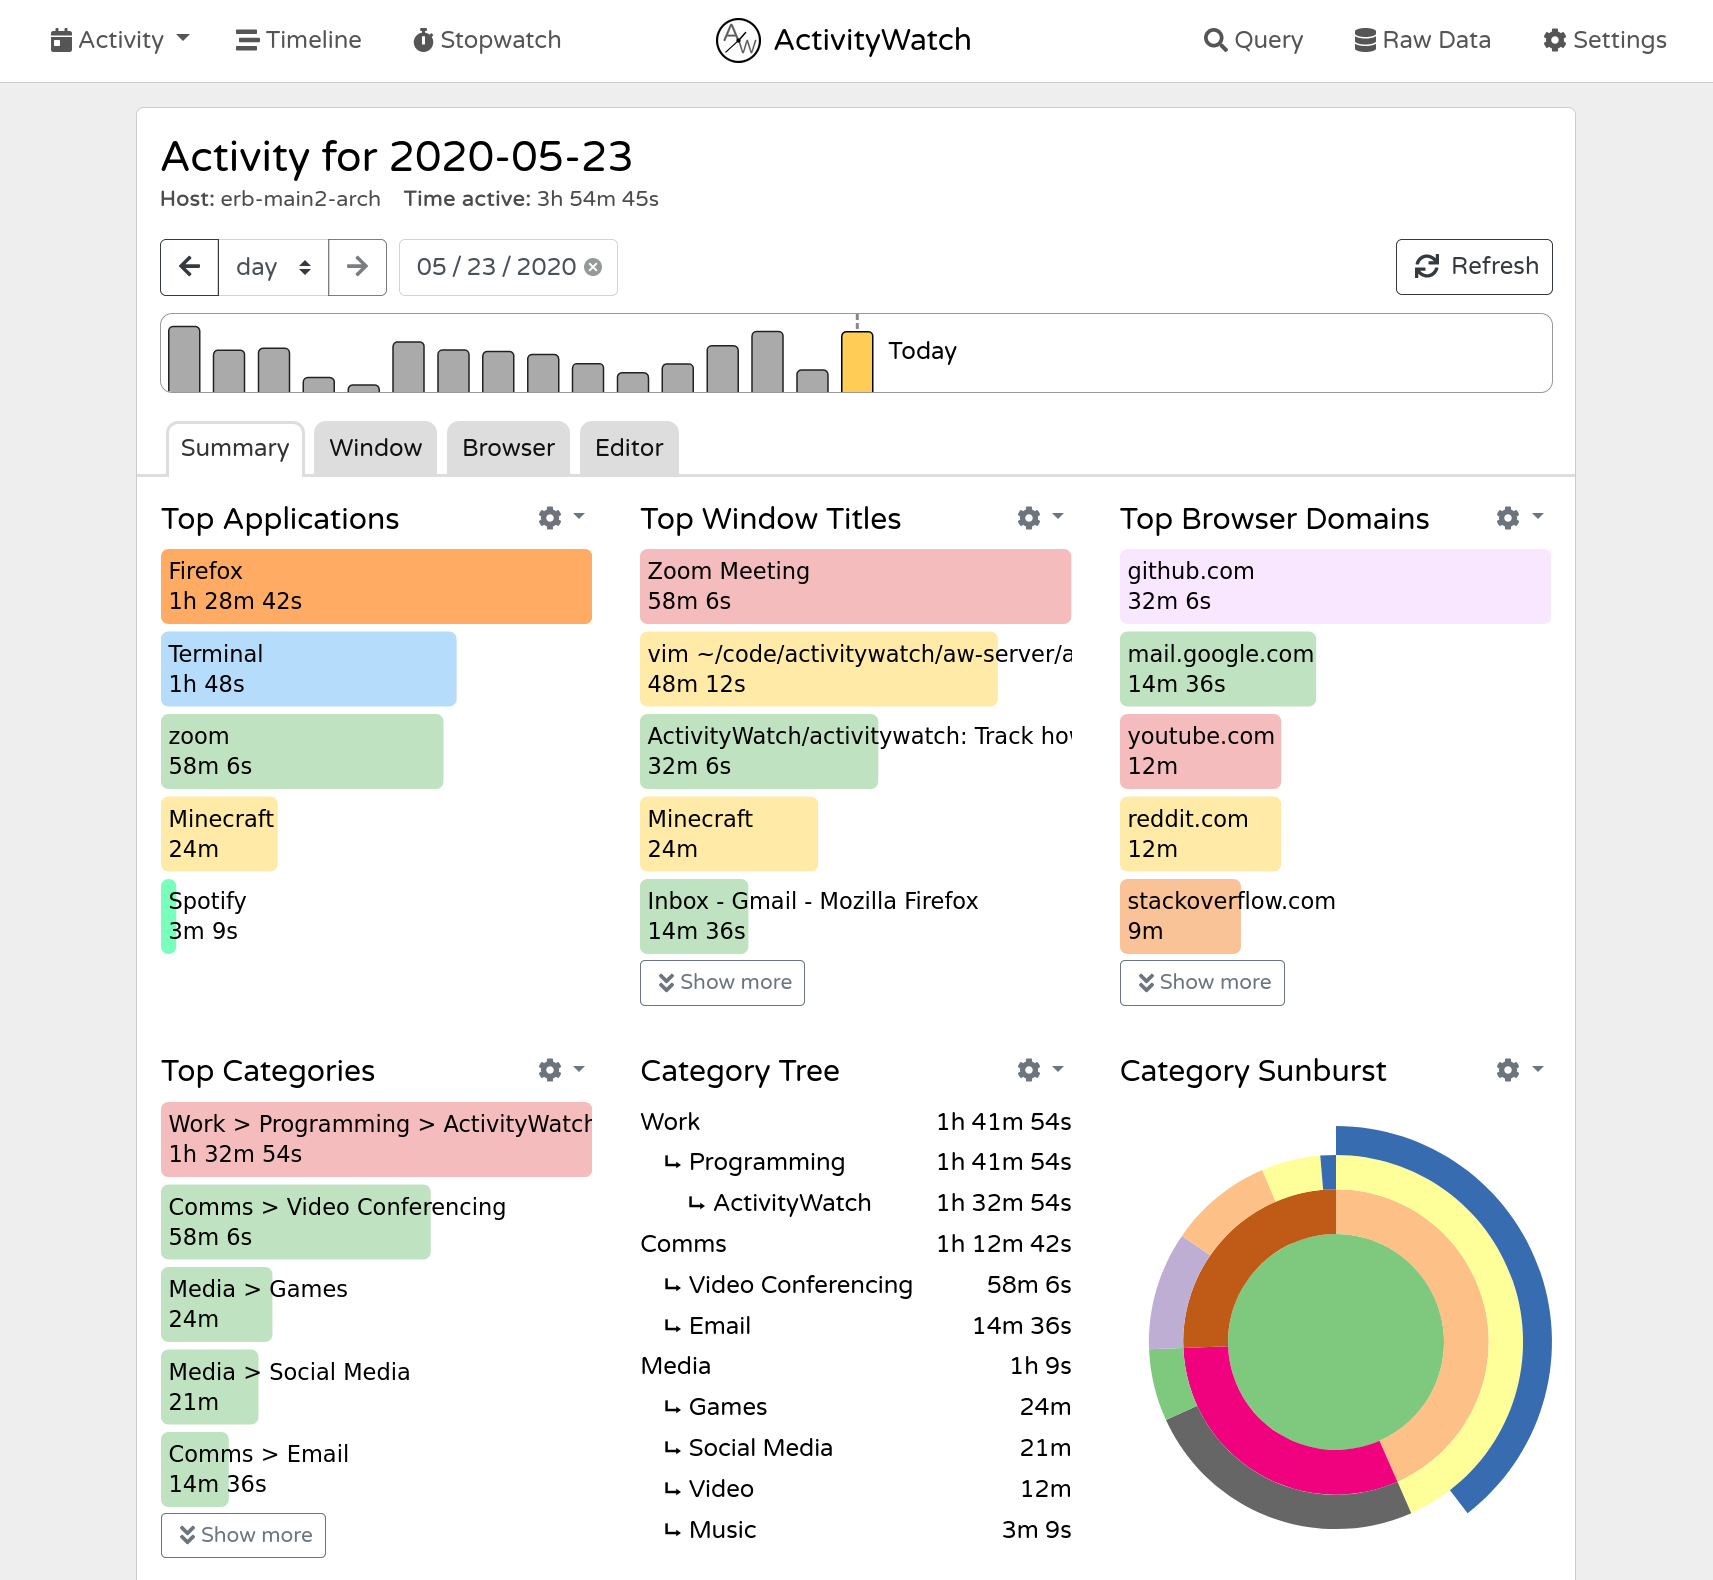
\includegraphics[width=12cm]{img/screenshot-aw-activity.png}
        \caption{ActivityWatch activity dashboard. Showing top applications, window titles, browser domains, and categories.}\label{fig:aw}
        \end{figure}

        ActivityWatch as a project was started in 2016 by the author of this thesis, with his brother Johan joining development soon after. It has since become a popular open source alternative to other time tracking software. It has received numerous contributions from users\footnote{Contributor statistics available at \href{https://activitywatch.net/contributors/}{activitywatch.net/contributors/}} and is approaching 100,000 downloads\footnote{Download statistics available at \href{https://activitywatch.net/stats/}{activitywatch.net/stats/}}.

        \todo[inline]{What more could I add about ActivityWatch? There should be relevant stuff in the docs, and in the slides I made way back.}

\subsection{EEG and low-cost biosensors/functional brain imaging}

    Functional brain imaging methods such as fMRI, fNIRS, and EEG, have been used to study the relationship between cognitive or physical activity, and brain activity~\cite{floyd_decoding_2017}\cite{hong_classification_2015}\cite{fucci_replication_2019}. The more accurate methods such as fMRI are costly and inflexible/impractical for many uses.

    However, the recent availability of low-cost biosensors such as EEG, HEG, and fNIRS, enables studying brain activity during real-life tasks.

    But EEG is not without its limitations --- among them a notably low signal-to-noise ratio~\cite{mcfarland_eeg-based_2017}, as well as being difficult to use for discerning activity deeper in the brain~\cite{fahimi_hnazaee_localization_2020} --- yet these limitations have been overcome for many applications, like ERP experiments, and has even turned out prove sufficient for high-speed BCI applications through detecting visual evoked potentials (VEPs)~\cite{spuler_high-speed_2017}.

    To combat the low signal-to-noise ratio, machine learning methods have been employed with varying degrees of success. Examples from previous research include Convolutional Neural Networks (CNNs), which have been successful in classifying time series in general~\cite{zhao_convolutional_2017}, and EEG data in particular~\cite{schirrmeister_deep_2017}. As well as Hierarchical Convolutional Neural Networks (HCNNs), which have been used for EEG-based emotion recognition~\cite{li_hierarchical_2018}.

    \add[inline]{Separate sections for applications in BCIs vs neuroscience}

    \subsubsection{Cost reduction}

    The cost-reduction of EEG devices took hold in 2013, when OpenBCI ran the founding crowdfunding round on Kickstarter. During the campaign, they offered their 16-channel Cyton + Daisy board for \$549.\footnote{Fun fact: I funded them at one of the lower tiers back then.}\cite{noauthor_openbci_nodate}

    The commercialization of EEG towards a general audience was furthered by InteraXon with the release of the original Muse in 2016. Aimed at meditation practice, it was the first consumer-oriented EEG device on the market.

    More recently, projects like the FreeEEG32 offer a 32 channel board for only \$199, expected to ship in 2022.\cite{noauthor_freeeeg32_nodate}

    \subsubsection{Applications in neurolinguistics}

        EEG has found many applications in neurolinguistics, both to understand how the brain processes natural languages as well as programming languages~\cite{prat_relating_2020}.

         As an example it has been shown that it is possible to classify if a participant is reading code or prose using fMRI~\cite{floyd_decoding_2017}, which has been replicated using EEG and low-cost biosensors~\cite{fucci_replication_2019}. The ability to distinguish between these two tasks have been has been explained neurologically by the recruitment of different neural networks in the brain~\cite{ivanova_comprehension_2020}. 

        The code vs prose comprehension task has also been modified into a writing task studied under fMRI, to further shed light to the underlying brain activity. In one study it was found that code and prose writing are significantly dissimilar tasks for the brain, where prose writing engages brain regions associated with language in the left hemisphere while while code writing engages brain regions associated with attention, working memory, planning, and spatial cognition in the right hemisphere\cite{noauthor_neurological_nodate}. To study this with MRI, the authors had to use (develop?) an MRI-safe keyboard.

        As far as I know, code vs prose writing has not been studied with EEG\. However, using ActivityWatch and other tools we've developed in this thesis (like the input watcher) one can to distinguish wether the user is reading or writing, as well as wether they're working with code or prose, which enables studying the same activities in a naturalistic setting.

    \subsubsection{Applications in software engineering}

        \add[inline]{Applications to software engineers (Fucci and related stuff)}

    % https://docs.openbci.com/citations

    % List of functional brain imaging techniques:
    %  - fMRI
    %  - fNIRS
    %  - EEG
    %  - HEG

\subsection{Aim of the thesis}

    \todo[inline]{Make align with goaldoc}

    The primary aim of the thesis is to improve upon previous attempts~\cite{fucci_replication_2019} to classify whether the user is reading code or prose using EEG data. This is to be achieved by using better EEG equipment and state of the art analysis methods such as Riemannian geometry. A secondary aim of the thesis is to investigate whether the ability of EEG analysis to classify code vs prose comprehension generalizes across more activities, such as the wide variety of tasks engaged in during organic device use.

    Secondary aims of the thesis include:

    \begin{enumerate}
        \item Implementing a classifier for device activities from EEG data, during organic device use
        \item Improving open-source tools for EEG analysis
    \end{enumerate}

    \add[inline]{Insert stuff from goal document}

\subsection{Related work}

    A systematic mapping study has been published which seeks to review the usage of psychophysiological data in software engineering~\cite{vieira_usage_2021}.

    It has previously been shown that fMRI~\cite{floyd_decoding_2017} and EEG\cite{fucci_replication_2019} provides enough information to classify whether a subject is reading prose or code. However, accuracy with single-channel EEG has been found to be poor, and notably outperformed by a heart rate variability (HRV) monitor.

    % Here, we used functional magnetic resonance imaging to investigate two candidate brain systems: the multiple demand (MD) system, typically recruited during math, logic, problem solving, and executive tasks, and the language system, typically recruited during linguistic processing.
    Recently, it has been shown that the multiple demand (MD) system is typically recruited for code comprehension tasks, as opposed to the language system that is typically recruited during prose comprehension~\cite{ivanova_comprehension_2020}. This sheds light on the significant differences in how the brain processes code vs prose.

    In addition to purely studying comprehension (reading) code and prose, an 2020 fMRI study showed that there are indeed significant neurological differences between \emph{writing} code and prose as well~\cite{noauthor_neurological_nodate}.

    In software engineerig research, low-cost biosensors such as wristbands that measure electrodermal activity and heart-related metrics have been used for emotion detection, as a tool in studying developer productivity.

    \add[inline]{Insert mention of preprint that Fucci mentioned?}

\section{Theory}

\subsection{Electroencephalography (EEG)}

    Electroencephalography is a method used to measure the activity of neurons in the brain by recording the electrical activity on the scalp.

    As a non-invasive method it is widely used in medicine to diagnose and study a wide range of conditions, including epilepsy and sleep disorders.

    In research it has also found use in studying ``Event Related Potentials'', or ERPs, which are stereotypes responses to a stimulus. Common ERPs can be seen in Table~\ref{table:erps}.

    \begin{table}
        \begin{tabular}{ll}
            \toprule
            ERP & Description
            \\
            \midrule
            N170 & Elicited by processing of faces, familiar objects or words.
            \\
            N400 & Elicited by words and other stimuli.
            \\
            P600 & Elicited by hearing or reading grammatical errors and other syntactic anomalies.
            \\
            \bottomrule
        \end{tabular}
        \caption{Common ERPs}\label{table:erps}
    \end{table}

    Electrodes can be placed at different locations on the scalp, targeting different regions of the brain. The system used to position the electrodes is called the 10–20 system, and is the standard way to label electrode placements.

    \begin{figure}
        \begin{center}
            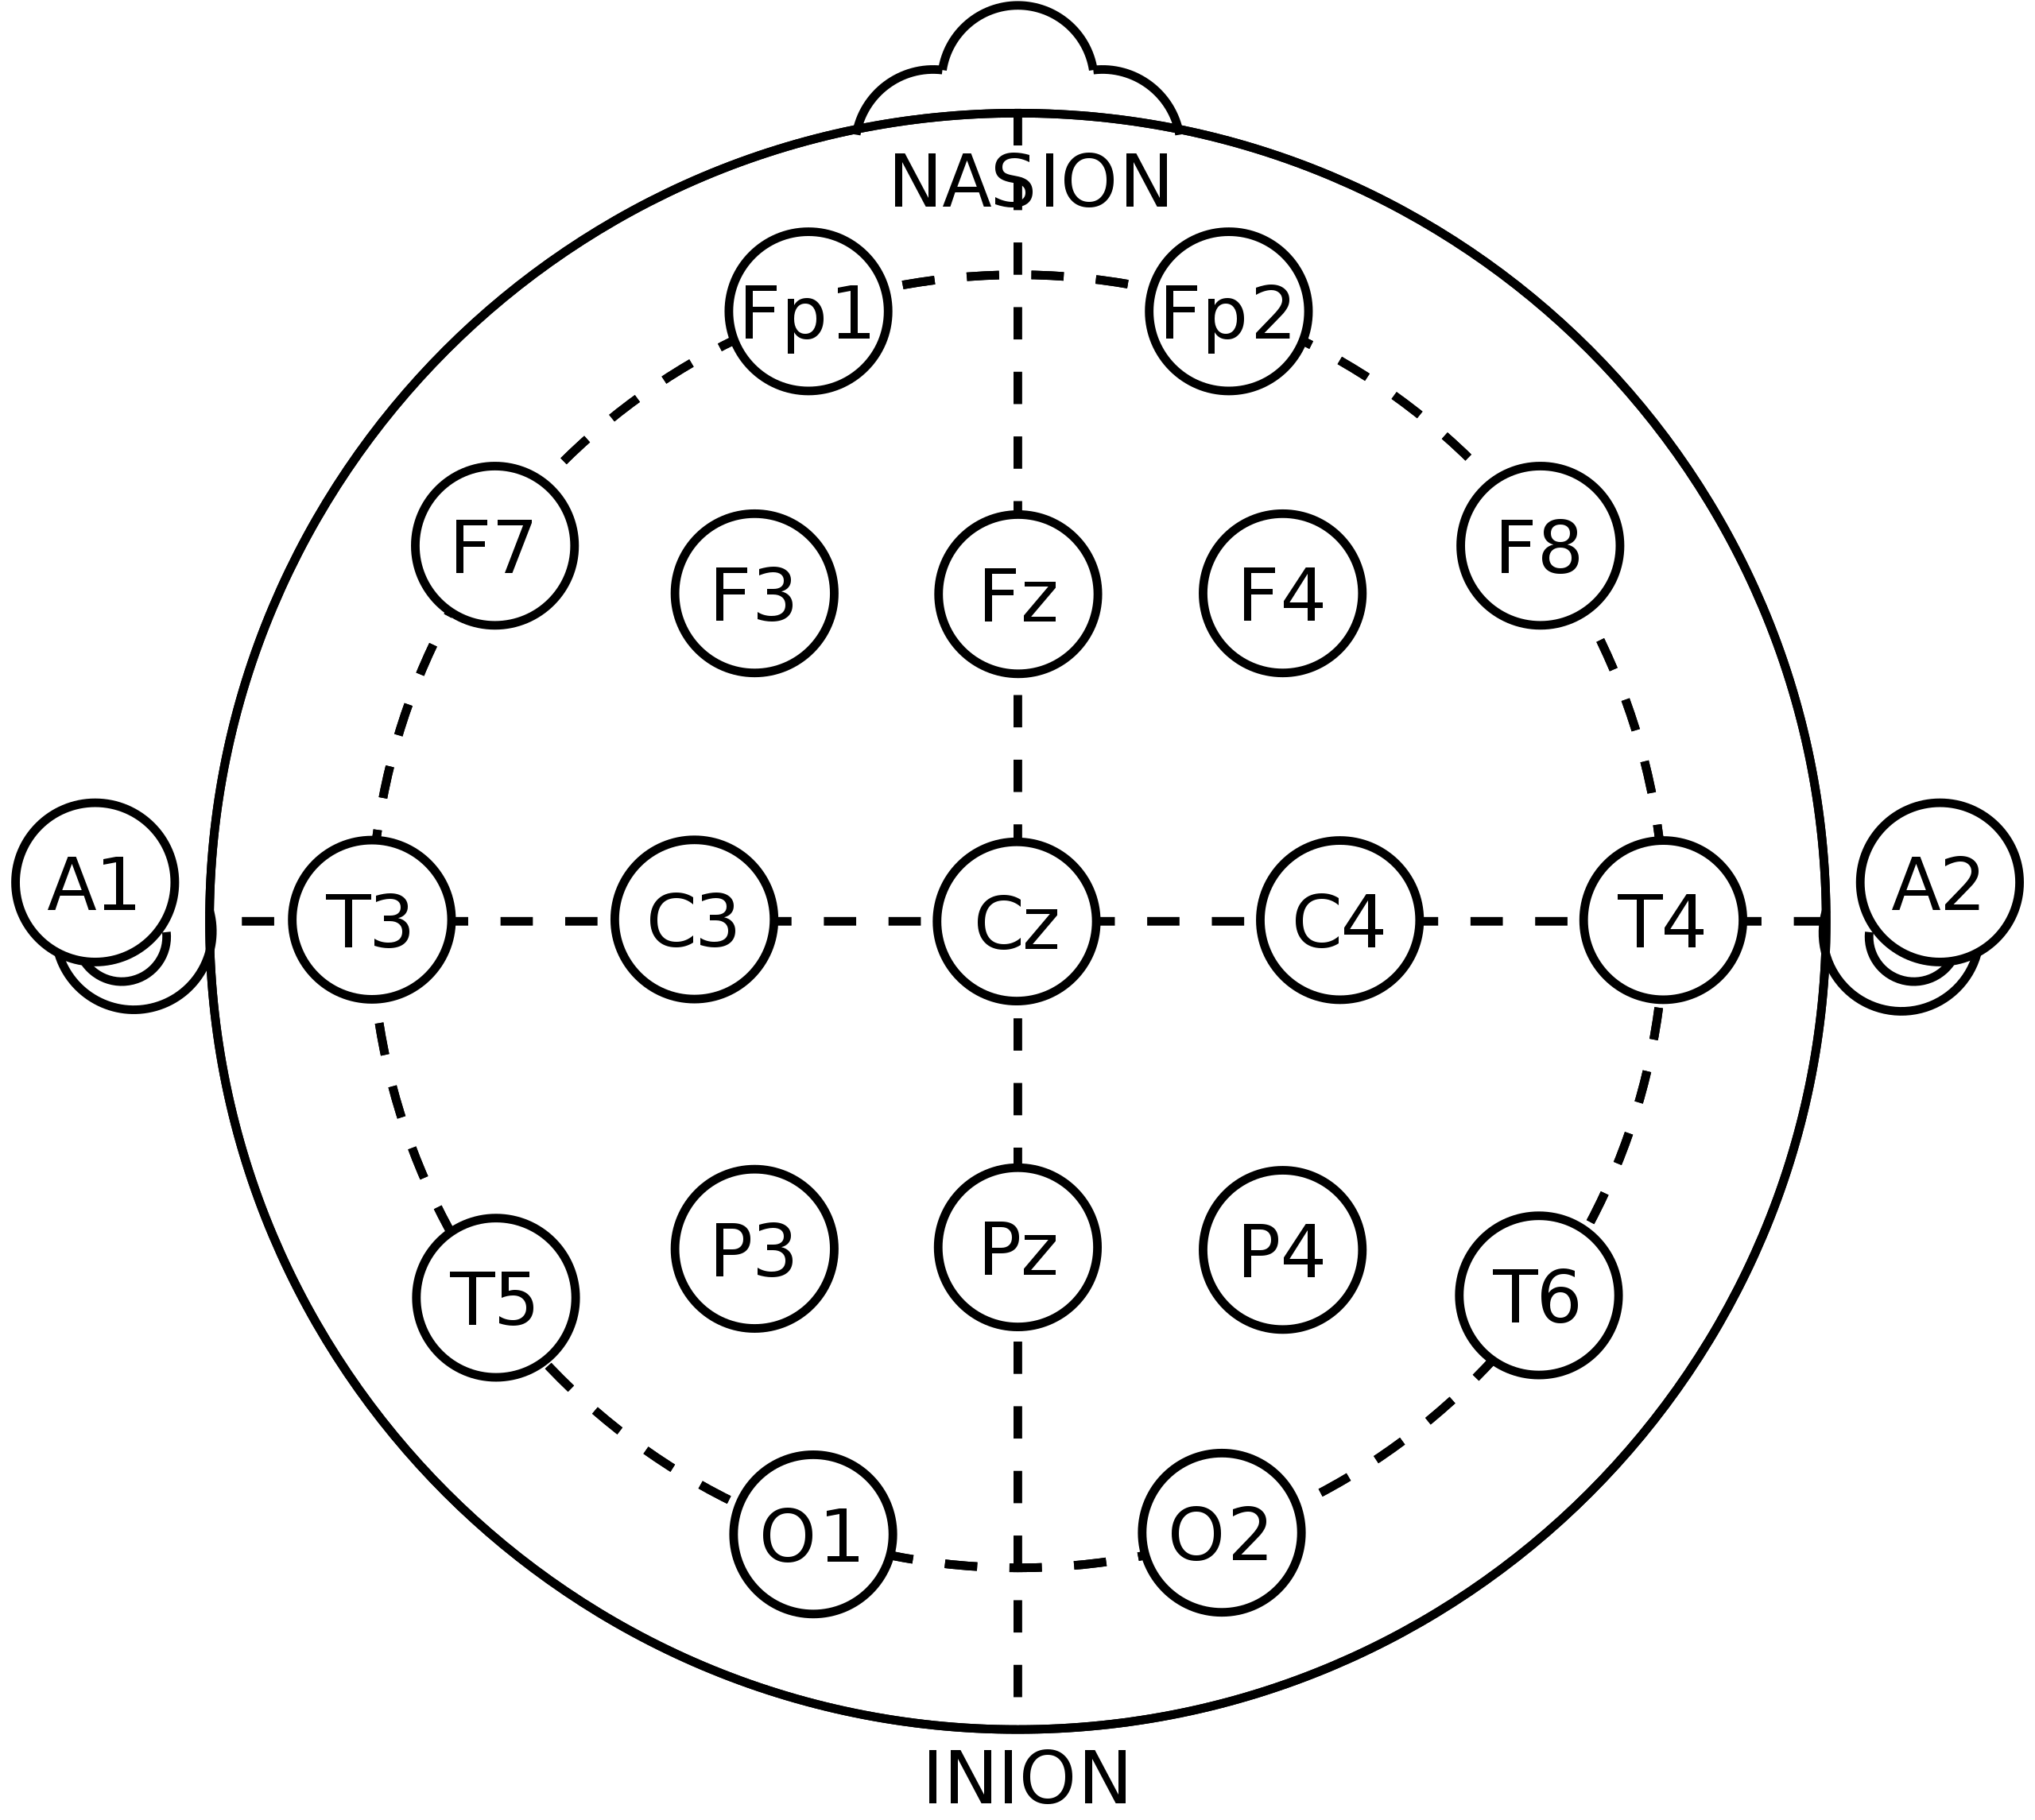
\includegraphics[width=10cm]{img/1020system.png}
        \end{center}
        \caption{The 10–20 system}\label{fig:1020}
    \end{figure}

    \add[inline]{Explain theory used, like theory of EEG, Riemannian geometry, etc}
    \add[inline]{Plots of raw EEG signal, PSD, PCA, etc}

    As measurements are taken on the scalp, neural activity of surface-level neurons, such as the cerebral (neo)cortex, can be expected to dominate the signal, which makes it difficult to use when studying systems deeper in the brain, such as the hippocampus. As an example of this, eye blinks are easily identifieable in the signal when electrodes are placed on the frontal cortex.

    \add[inline]{Mention need for bandpass filtering to get rid of powerline noise}

    \add[inline]{Plot of signal during eye blink}
    \add[inline]{Discuss some of the review articles on EEG/BCI/ML}

\subsection{Machine Learning}

    Machine learning on EEG data utilizes several domain-specific methods (which?) often similar to other methods seen applied to general time-series data.

    Among these we find methods like bandpass filtering, windowing, spectral density estimation, and the computation of covariance matrices to find interdependencies between channels.

    Common methods used in analysis and classification of EEG data include Linear Discriminant Analysis (LDA), Common Spatial Pattern (CSP) filters.

    With the use of these methods, we can compute features to use when training our classifiers.

    The underlying ML algorithms themselves are often off-the-shelf logistic regression, with some domain adaptations found in more complex models like neural networks.

    \add[inline]{Formulas}

    \subsubsection{Riemannian geometry}

        \add[inline]{Explanation of Riemannian geometry, from \href{https://colab.research.google.com/drive/1y9tq7-lJwusxtVgpB38y-p1pYw7hg0iu}{this tutorial we're working on}, perhaps it should go in the Background/Theory section though?}

        The Riemannian distance measure for two symmetric positive definite matrices (such as a covariance matrix) is:~\cite{grafarend_metric_2003}

        \[ d(A, B) = \sqrt{\sum_{i=1}^{n} \ln^2 \lambda_i (A, B) } \]

    \subsubsection{Neural networks}

        Many state-of-the-art models in the field of EEG are deep-learning based models, usually employing convolutional neural networks (CNNs).

\chapter{Method}

We start by deciding on an EEG device to use, we then collect data for both the controlled and naturalistic experiments. Once the data has been collected, we perform data labelling, transformation, and cleaning. 

Finally, we train classifiers using various machine learning methods, in particular ones based on Riemannian geometry. We also train a classifier based on bandpower-features as a baseline reference.

An overview of the process is presented in Figure~\ref{fig:method}.

\begin{figure}[h]
    \centering
    \includegraphics[width=14cm]{img/method.png}
    \caption{Overview of the process for the two separate tasks.}\label{fig:method}
\end{figure}

\begin{minipage}{\textwidth}
The method for our controlled experiment mimics Fucci et al.~\cite{fucci_replication_2019} with some differences (seen in Table~\ref{table:compare-method}): 

\begin{itemize}
        \item We use EEG exclusively.
        \item We used a different device.
        \item We have a smaller \& less diverse sample.
        \item We have reimplemented the task in eeg-notebooks.
        \item We have used the original prose-review stimuli by Floyd et al.~\cite{floyd_decoding_2017}.
\end{itemize}

    Some of these differences are motivated and discussed further later in the report, especially in Section~\ref{section:threats}.
\end{minipage}

% Comparing to Fucci and original study
\begin{landscape}
    \rowcolors{4}{gray!25}{white}
\begin{table}
    \begin{center}
        \begin{tabular}{llll}
            \toprule
            \multirow{2}{*}{\textbf{Setting}} & \multicolumn{3}{c}{\textbf{Study}} \\
            \cmidrule(lr){2-4}
            & \makecell[c]{\textbf{This study}} & \makecell[c]{\textbf{Fucci et al.} (2019)} & \makecell[c]{\textbf{Floyd et al.} (2017)} \\
            \midrule
            Experiment site & Lund Univ. (Sweden) & Univ.\ of Bari (Italy) & Univ.\ of Virginia (USA)  \\
            \# Participants & 9 & 28 & 29 \\
            Participants experience & Grads & Undergrads & Grads \& Undergrads \\
            \# Tasks & Variable & 36 tasks & 27 tasks \\
            Task type & \makecell[l]{Code comprehension \\ Prose review} & \makecell[l]{Code comprehension \\ Prose comprehension} & \makecell[l]{Code comprehension \\ Code review \\ Prose review} \\
            Physiological signal & Neural & \Gape[0pt][2pt]{\makecell[l]{Neural \\ Skin \\ Heart}} & Neural \\
            Physiological measure & EEG & \makecell[l]{EEG \\ EDA \\ HR, HRV, BVP} & BOLD \\
            Device & Muse S & \Gape[0pt][2pt]{\makecell[l]{BrainLink Headset \\ Empatica wristband}} & fMRI \\
            Classifier & Riemannian geometry & 8 algorithms & Gaussian Process \\
            Classifier validation & LORO-CV & \Gape[0pt][2pt]{\makecell[l]{LORO-CV \\ Hold-out}} & LORO-CV \\
            Classifier metric & Balanced accuracy (BAC) & Balanced accuracy (BAC) & Balanced accuracy (BAC) \\
            \bottomrule
        \end{tabular}
        \caption{Comparison of this study's method with previous studies.}\label{table:compare-method}
    \end{center}
\end{table}
\rowcolors{2}{}{}

\end{landscape}
\rowcolors{2}{}{}

% Equipment
\section{Devices}
    
    In this section we will briefly describe the different EEG devices we have worked with, and their differences.

    We experimented with several devices but eventually settled on the Muse S. The motivation for choosing the Muse S was mainly due to comfort and ease of use. 

    The other devices considered included the OpenBCI Cyton (with the Ultracortex headset), and the Neurosity Crown.\footnote{Earlier in the work, before we received the Crown, we were also generously gifted a Neurosity Notion DK1 to get a head start.} 

    In our framework, we have implemented support all of the headsets mentioned (and more), such that future work can use whichever device is desired.

    \vspace{0.5cm}
    \begin{table}[H]
    \centering
    \begin{tabular}{llcrr}
        \toprule
        Manufacturer
        & Device
        & Channels
        & Sampling rate
        & Comfort
        \\
        \midrule
        InteraXon
        & Muse S (2020)
        & 4
        & 256Hz
        & High
        \\
        Neurosity
        & Crown (2021)
        & 8
        & 256Hz
        & Medium
        \\
        OpenBCI
        & Cyton (2013) + Ultracortex
        & 8--16
        & 125--250Hz
        & Low
        \\
        \bottomrule
    \end{tabular}
    \caption{Devices used}\label{table:devices}
\end{table}

    \vspace{0.5cm}

    \begin{minipage}{\textwidth}
        \paragraph*{Muse S}
        The Muse S is a 4-channel EEG headband with electrodes at TP9, AF7, AF8, and TP10 (using the modified 10--10 system, seen in Figure~\ref{fig:1010}), with the reference electrode at Fpz~\cite{krigolson_choosing_2017}. Its main advantage is its very comfortable form-factor and long battery life. It's limited by its channel count and electrode placement. It connects using Bluetooth.

        \begin{figure}[H]
            \centering
            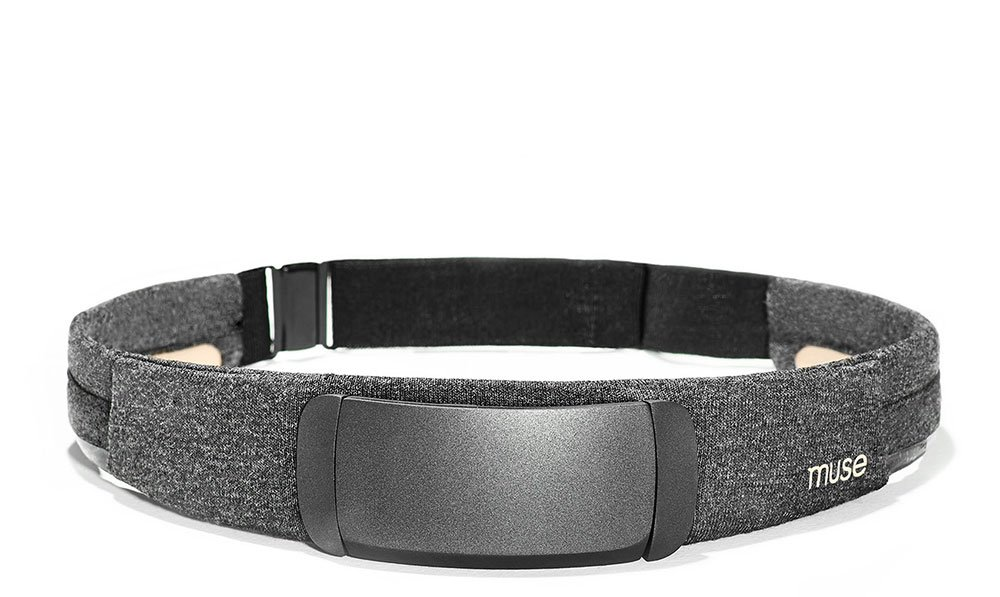
\includegraphics[trim=0 0 0 200,clip,width=100mm]{img/Muse-S.jpg}
            \caption{Muse S}\label{fig:museS}
        \end{figure}
    \end{minipage}

    \begin{minipage}{\textwidth}
        \paragraph*{OpenBCI Cyton}
        The OpenBCI Cyton is a 8-channel EEG board. It is commonly used with the partly 3D-printable OpenBCI Ultracortex Mark IV headset, which allows for flexible electrode placement. OpenBCI also offers an expansion board, the Daisy, which adds 8 additional channels. It connects using Bluetooth.

        %The main disadvantage is the comfort of the Ultracortex headset, which makes it difficult to use for longer sessions. A wet-cap headset would address this, but that has other disadvantages, like being messy and time-consuming.

        \begin{figure}[H]
            \centering
            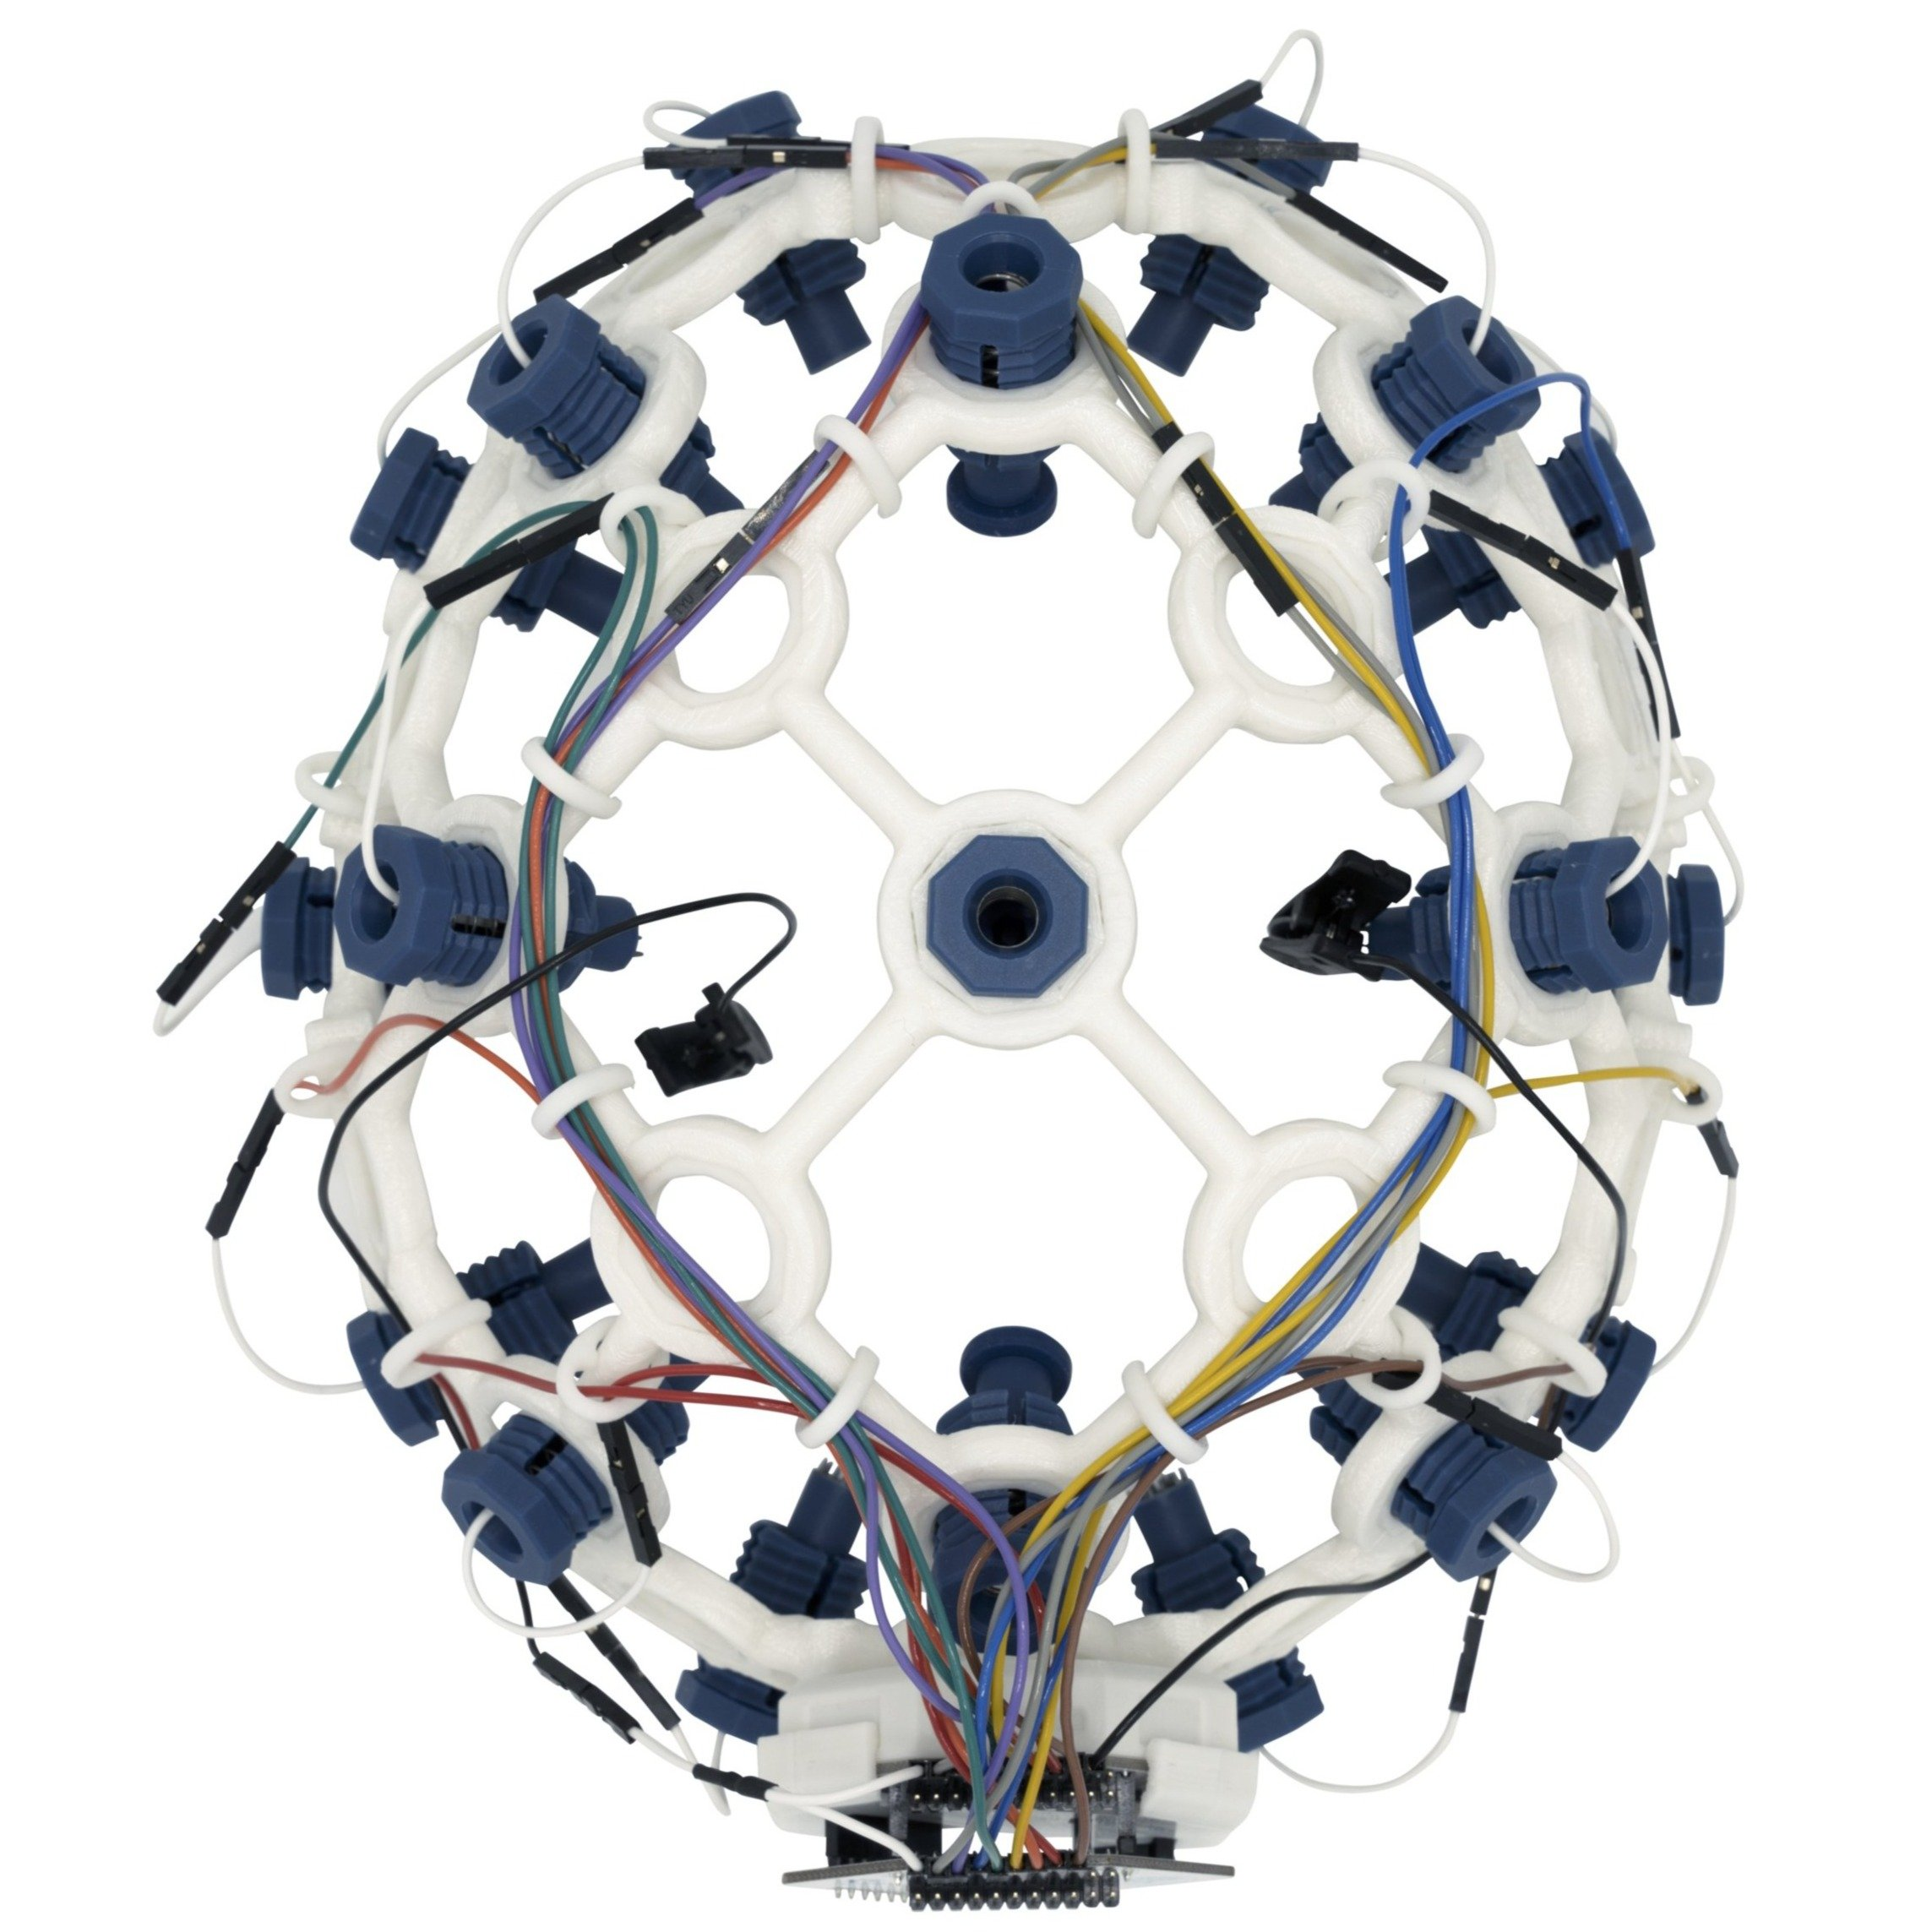
\includegraphics[width=80mm]{img/openbci-cyton.jpg}
            \caption{OpenBCI Cyton + Daisy with Ultracortex Mark IV}\label{fig:cyton}
        \end{figure}
    \end{minipage}

    \vspace{1cm}

    \begin{minipage}{\textwidth}
        \paragraph*{Neurosity Crown}
        The Neurosity Crown is a 8-channel EEG headset. It runs Linux on a quad-core CPU and 1GB RAM, and connects via WiFi. It has electrodes placed at CP3, C3, F5, PO3, PO4, F6, C4, CP4. Reference and bias electrodes at T7 and T8.

        \begin{figure}[H]
            \centering
            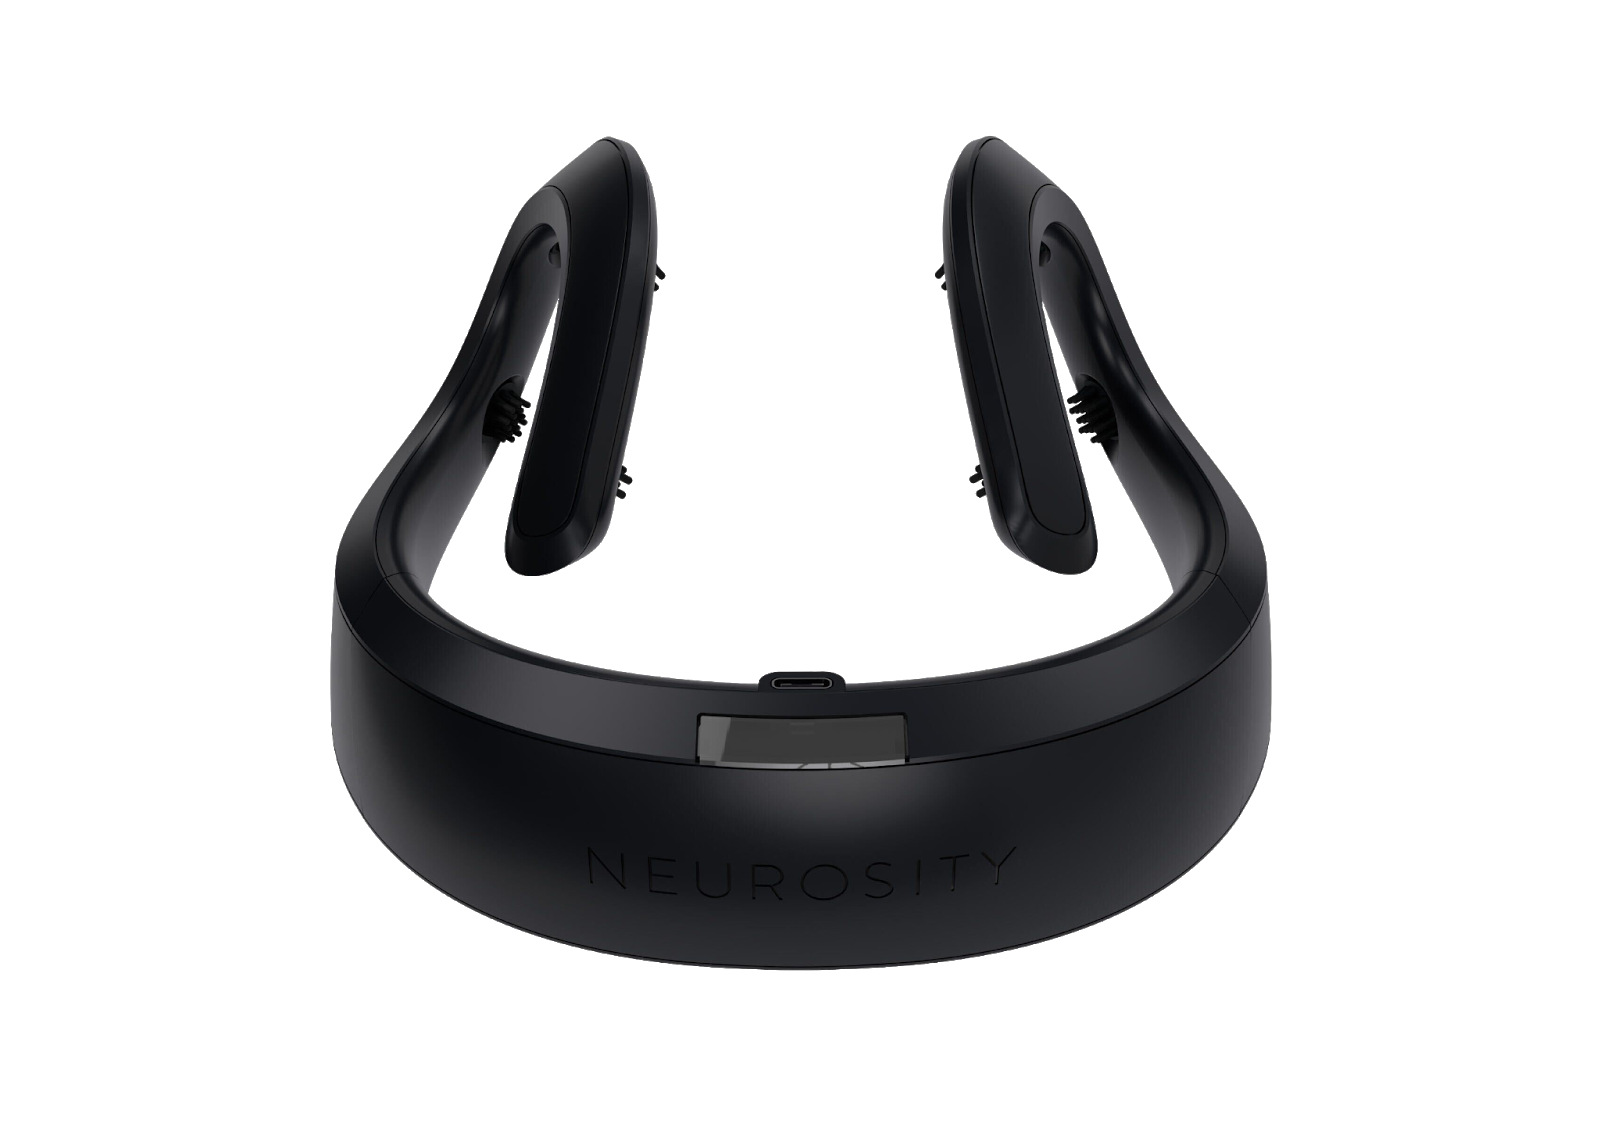
\includegraphics[trim=0 100 0 100,clip,width=100mm]{img/crown-1.png}
            \caption{Neurosity Crown}\label{fig:crown}
        \end{figure}
    \end{minipage}

\pagebreak
\section{Collection}

We need two types of data for the experiments: EEG data, and labels. For the controlled experiment, our labels are whether the stimuli is code or prose. For the naturalistic use experiment, our labels are the device usage categories.

To collect data for the controlled experiment, we:

\begin{enumerate}
    \item Set up the EEG equipment
    \item Use eeg-notebooks to present the stimuli, and record the time markers of when the stimuli changed as labels.
\end{enumerate}

To collect data for the naturalistic use experiment, we:

\begin{enumerate}
    \item Set up the EEG equipment
    \item Configure ActivityWatch to collect device usage data
\end{enumerate}

    \subsection{Collection of EEG data}

        EEG data was collected for the controlled experiment and during naturalistic device use. For both conditions, code from the open source \texttt{eeg-notebooks}~\cite{barachant_eeg-notebooks_2020} was adapted to record the raw EEG stream into a CSV file.

        Depending on the device used we require certain software to connect to the devices. We used muse-lsl for the Muse S~\cite{muse-lsl} which in turn uses Lab Streaming Layer. To support OpenBCI and Neurosity devices we used brainflow~\cite{noauthor_brainflow_2020}.

        We have developed `brainwatch', a command-line interface tool, to help us connect to and record from EEG devices. To connect \& record from an EEG device, we can simply run:

        \inputminted{bash}{figures/brainwatch-example.txt}

        We can then check signal quality with \mintinline{bash}{brainwatch check}, or run \mintinline{bash}{brainwatch plot} to plot the raw signal.

        Alternatively, we can plot using muse-lsl's built-in plotting functionality: \mintinline{bash}{muselsl view -b Qt5Agg} (seen in Figure~\ref{fig:muselsl-signal}).

        \subsubsection*{During naturalistic device use}\label{section:collect-eeg-naturalistic}

            For the naturalistic device use conditions, we used the Muse S due the superior comfort and ease of use compared with the alternatives, making it especially suitable for long recordings.\footnote{A wet electrode cap system was also considered, but was not used due to being inconvenient to setup.}

            For this experiment we use a single-subject (the experimenter). The subject was asked to go about their usual device activities, often consisting of a mix of work (writing code, writing prose, email) and leisure (watching YouTube, reading Twitter).
            
            We collected approximately 5 hours of EEG data during natural device use, and use the classes defined in Section~\ref{section:collect-usage} as labels for the data.

        \subsubsection*{During code vs prose comprehension task}

            For the controlled condition, we ended up using the Muse S as well due to the comfort and ease of setup.

            We have 9 subjects, sampled by convenience. The subjects were 8 males and one female. Most are in their late 20s or early 30s, except two who are in their 40s.

            The experiment consists of presenting images with code or prose comprehension tasks, seen in Figure~\ref{fig:tasks}. These images are from previous studies on code vs prose comprehension by Floyd et al.~\cite{floyd_decoding_2017} and Fucci et al.~\cite{fucci_replication_2019}. 

            \begin{figure}[H]
    \centering
    \begin{tabular}{cc}
        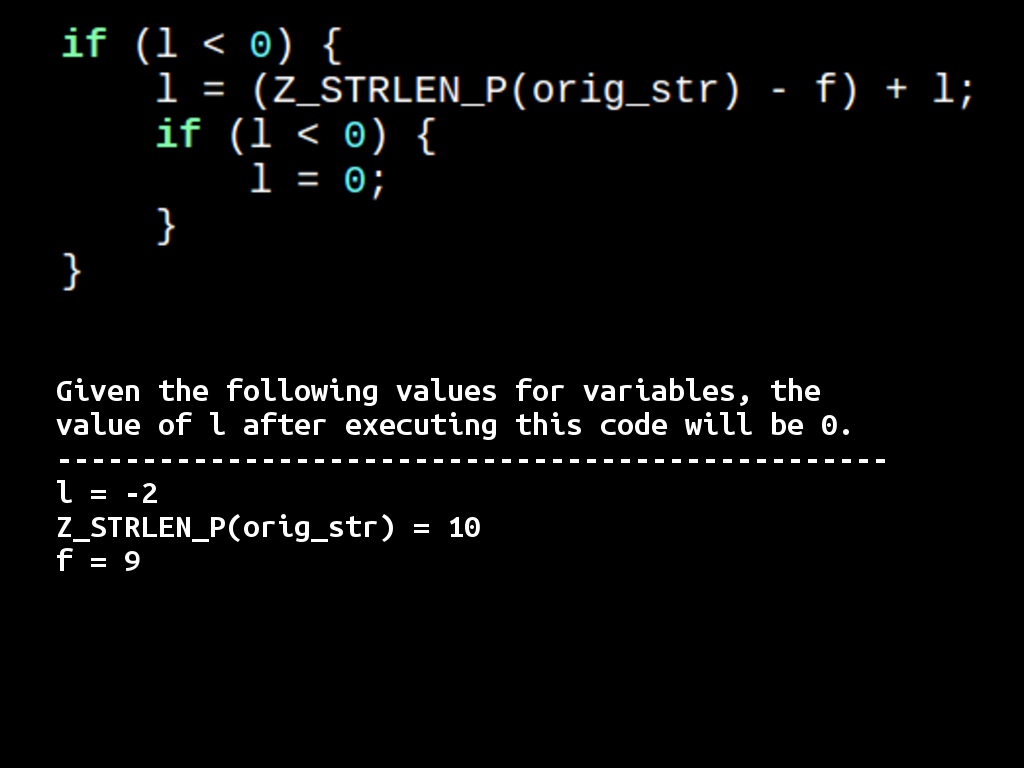
\includegraphics[trim=25 160 0 0,clip,width=0.45\linewidth]{img/final-1-1.png}
        &
        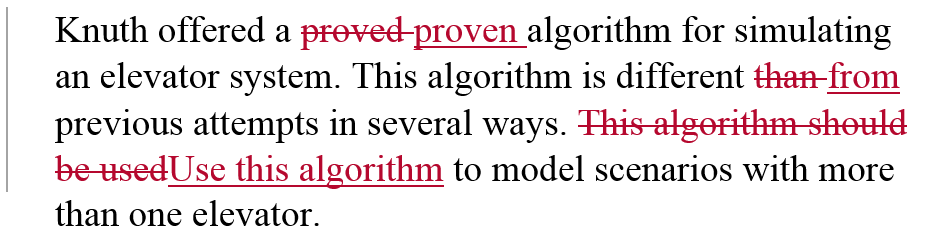
\includegraphics[trim=20 0 20 0,clip,width=0.45\linewidth]{img/bugs_1.PNG}
        \\
        (a) Code comprehension
        &
        (b) Prose review
    \end{tabular}
    \caption{Sample of the tasks used as stimuli.}\label{fig:tasks}
\end{figure}


            We note that Fucci et al.~modified the prose comprehension images from the original review-like task to become more comprehension-like, arguably better suited for the task (seen in Figure~\ref{fig:prose-comp-fucci}). However, due to the modified images being in Italian, we have used the original prose review images by Floyd et al.

            \begin{figure}[H]
                \centering
                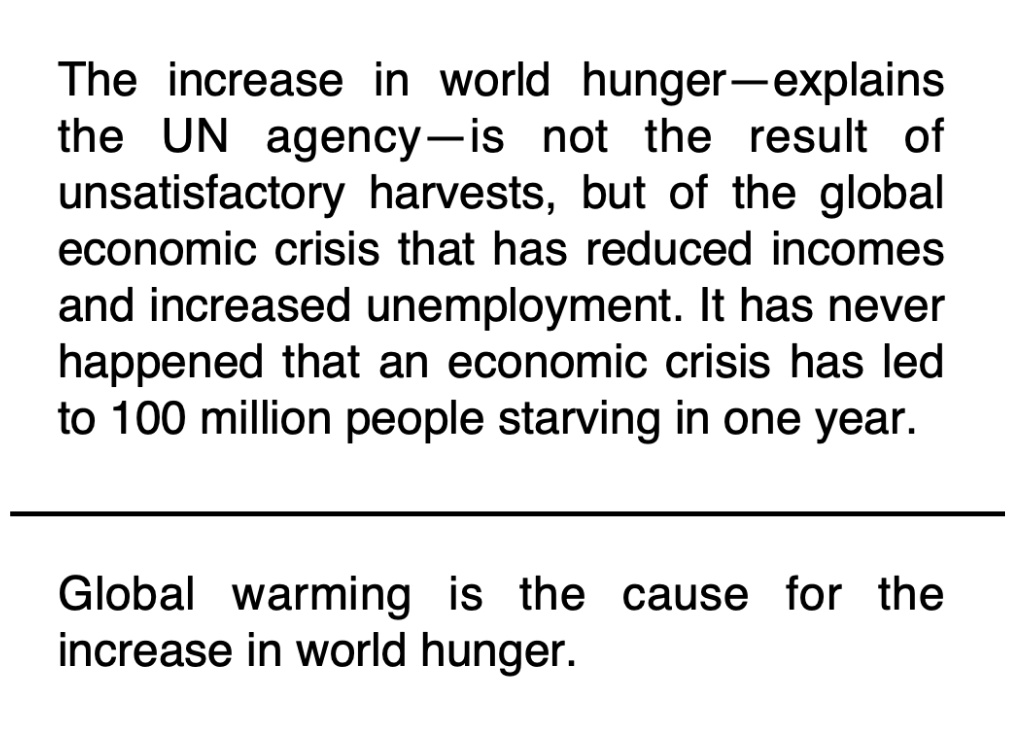
\includegraphics[width=90mm]{img/prose-comprehension.png}
                \caption{Sample of the prose comprehension task used by Fucci et al. (translated from Italian).}\label{fig:prose-comp-fucci}
            \end{figure}

            We implemented the task in eeg-notebooks~\cite{barachant_eeg-notebooks_2020}, which uses previously mentioned libraries for data collection as well as PsychoPy~\cite{peirce_psychopy2_2019} to present the stimuli.

            Before each run, the subject was asked about their gender, age, handedness, and software development experience (specifically experience with C/C++). For good measure, we also asked if the subject had consumed caffeine the hours prior to the experiment.

            After these questions we put the devices on and ensure we get good signal by inspecting it in real time with the viewer provided by muse-lsl (seen in Figure~\ref{fig:muselsl-signal}). The viewer itself does simple bandpass filtering between 3--40Hz, and the signal quality is indicated by the standard deviation of the filtered signal.

            The stimuli images were presented in random order, for all subjects except subject \#1 due to experimenter error (seen in Figure~\ref{fig:timebars}). For each stimuli the subject is asked to answer True/False to the questions posed by the code comprehension stimuli, or Correct/Incorrect for the prose review images. There is a short rest period of 5s between each stimuli. Each experiment run lasted between 10--25 minutes, depending on subject tiredness (subjects were asked to stop when tired).

    \vfill
    \pagebreak
    \subsection{Collection of device activity data}\label{section:collect-usage}

        All device activity is collected using the automated time tracker ActivityWatch~\cite{bjareholt_activitywatch_2020-1}.

        \begin{minipage}{\textwidth}
        ActivityWatch collects data through modules called watchers which report to the ActivityWatch server. It comes with two watchers by default:

        \begin{itemize}
            \item aw-watcher-window, tracks the active window and its title
            \item aw-watcher-afk, tracks if the user is active or not by observing input device activity
        \end{itemize}
        \end{minipage}

        We have also built a custom watcher, aw-watcher-input, to track metrics of mouse and keyboard activity. It tracks by listening to mouse and keyboard events and records the distance in pixels the mouse moves and the number of key presses (but not which key was pressed). Every second this is bundled into an event, the values are reset, and then it continues with the next event. It was inspired by similar functionality in Andrej Karpathy's ulogme~\cite{karpathy_ulogme_2016}.

        A limitation that we have to consider is that the window watcher uses a polling method to track the active window, with a default poll time of 1 second. This means that we can not rely on the timestamps to mark the exact time the window became active/inactive.

        The data from ActivityWatch is processed and categorized such that the resulting data has the 3 columns \mintinline{text}{start, stop, class}. The class is determined by a regular expression that matches on window titles and URLs. For example, the regular expression \mintinline{text}{GitHub|github.com} could be used to match GitHub use.

We chose a few classes for analysis, seen in Table~\ref{table:activity-classes}. Among them we have the classes \emph{Programming} and \emph{Writing}, to see if we can separate these activities in a natural setting.

\begin{table}[h]
    \centering
    \begin{tabular}{ll}
        \toprule
        \textbf{Activity} & \textbf{Regular Expression} \\
        \midrule
        Programming & \texttt{[.](py|rs|js|ts)} \\
        Writing & \texttt{[.](tex|md)} \\
        Twitter & \texttt{Twitter|twitter.com} \\
        YouTube & \texttt{YouTube|youtube.com} \\
        \bottomrule
    \end{tabular}
    \caption{Activity classes used to label EEG data.}\label{table:activity-classes}
\end{table}

\begin{figure}[h]
\begin{minted}{text}
start,               stop,                class
2020-09-20 13:32:51, 2020-09-20 13:34:09, Twitter
2020-09-20 14:44:08, 2020-09-20 14:46:11, YouTube
2020-09-21 09:49:04, 2020-09-21 09:49:35, GitHub->Issues
2020-09-21 09:51:32, 2020-09-21 09:52:23, Programming
2020-09-21 10:20:18, 2020-09-21 10:21:05, Writing
\end{minted}
    \caption{Examples of labeled time windows, collected and categorized with ActivityWatch}\label{code:class-csv}
\end{figure}

\vfill
\pagebreak
\section{Analysis}

    For classification and analysis, we used common open source Python libraries for data analysis, like numpy~\cite{harris2020array}, pandas~\cite{reback2020pandas}, and scikit-learn~\cite{scikit-learn}. In addition, we used less common libraries tailored specifically for working with EEG data, such as MNE~\cite{noauthor_mne-python_2020}, pyriemann~\cite{alexandre_barachant_2020_3715511}, and YASA~\cite{vallat_yasa_2020}.

    \subsection{Labelling}
        When labeling our data we define two levels of granularity: epochs and windows.

        An epoch is a single trial, such as a single stimuli image, which can have variable length due to the experiment setup where the subject decides when to move on to the next stimuli. We label epochs using markers from our experiments.

        A window is a fixed-duration slice of an epoch, such that each window matrix has the same dimensions. This enables us to more easily compute various features which require matrices to be of the same dimension. Windows inherit the label of the epoch from which they belong.

        For the naturalistic device use experiment, we split the EEG data into epochs using the categories assigned by our ActivityWatch script.

        For the controlled experiment, we split the EEG data into epochs using the trial markers, resulting in one epoch per stimuli.

    \subsection{Data transformation}\label{section:transform}

        In order to classify the epochs, which have variable length due to each subject taking a different amount of time to answer each trial, we split each epoch into a fixed-duration window. After some experimentation we found \SI{5}{\second} to be a suitable window size. Once we have our fixed-duration windows, we can use them to train our model and classify new samples.

        Dimensions of each epoch matrix: \[ (n_{\mathrm{samples}}, n_{\mathrm{channels}}) \]

        Where $n_{\mathrm{samples}}$ is the total number of samples for the epoch (variable-length), and $n_{\mathrm{channels}}$ is the number of channels (4 for the Muse S).

        Since the matrix has variable dimensions for each epoch, we split it into \SI{5}{\second} windows, which at the 256Hz sampling frequency of the Muse gives us 1280 samples per window.

        Dimensions of the window matrix: \[ (n_{\mathrm{windows}}, n_{\mathrm{channels}}, 1280) \]

        We experimented with different windowing methods to augment the data, but we ultimately decided against using them, as the methods did not seem to contribute to the performance of trained classifiers.

    \subsection{Data cleaning}

        We reject samples that either:

        \begin{enumerate}
            \item Do not have an assigned class
            \item Have a bad signal quality (as indicated by a signal variance $>40$)
            \item Are too short due to missing samples (such that a 5s window cannot be constructed)
        \end{enumerate}

        The exact number of samples rejected by each cleaning step, as well as the exact parameters used, can be viewed in the code notebooks published alongside this report.

        We also perform bandpass filtering between \SI{3}{\hertz} and \SI{40}{\hertz} to eliminate powerline noise. We can see the results of the bandpass filtering in Figure~\ref{fig:signal-unfiltered} and~\ref{fig:signal-filtered}.

    \subsection{Classification pipelines}

        In this section we describe our classification pipelines which use two different approaches:

        \begin{enumerate}
            \item Use bandpower features to train a common classifier algorithm (such as logistic regression, support vector machines, or random forests).
            \item Use Riemannian methods to work with distances between covariance matrices by using the Riemannian metric, and then apply a common classifier algorithm.
        \end{enumerate}

        \subsubsection{Bandpower-based}

            Bandpower features are simple and commonly used in EEG research for many tasks, including the paper by Fucci et al we seek to improve upon~\cite{fucci_replication_2019}. 

            As a benchmark reference, we implemented classifiers which solely used bandpower features as input, to gain information of how much any improvement from classifier performance is likely due to better EEG equipment versus how much is due to from improved analysis methods.

            To compute this feature, we utilized the bandpower function provided by YASA~\cite{vallat_yasa_2020}. The implementation estimates the power spectral density using Welch's method for each channel, and bins them by their associated frequency band (seen in Table~\ref{table:freq-bands}).

            To further enrich our feature vector, we can use ratios between two frequency bands. As this is what Fucci et al.\ did, we do the same.

            Finally, the pipeline trains 3 models using either logistic regression, support vector machines, or random forests.

        \subsubsection{Riemannian geometry}

            The state of the art in many EEG classification tasks involves the use of Riemannian geometry (described in Section~\ref{section:riemannian-theory}). For this, we used the open source \texttt{pyriemann} library by Alexandre Barachant\footnote{First author of the original paper to apply Riemannian geometry to EEG~\cite{barachant_classification_2013}}.

            Our final pipeline is defined by:

\begin{minted}{python}
from sklearn.pipeline import make_pipeline
from sklearn.linear_model import LogisticRegression
from pyriemann.estimation import Covariances
from pyriemann.spatialfilters import CSP
from pyriemann.tangentspace import TangentSpace

clf = make_pipeline(
    Covariances(),
    CSP(4, log=False),
    TangentSpace(),
    LogisticRegression(),
)
\end{minted}

            We do not perform any hyperparameter optimization.

    \begin{comment}
    \subsection{Neural Networks}

        \change[inline]{Future work!}

        One of the classifiers we want to train is a neural network. We use braindecode~\cite{schirrmeister_deep_2017}\cite{noauthor_braindecode_2021}, a neural network library for EEG data that uses PyTorch and integrates it with scikit-learn through skorch.

        The networks provided by braindecode are convolutional\ldots
    \end{comment}

    \subsection{Performance scoring}

        Previous studies have used \emph{balanced accuracy} (BAC) scoring with LORO validation to evaluate model performance. To be able to compare results to previous studies, we do the same. 

        BAC deals with imbalanced datasets by evaluating the performance of the classifier on each class and combining them into a single number. It is defined as the average of recall obtained on each class, or equivalently for a binary classifier, the average of the classifier sensitivity and specificity. 

        For a binary classifier, a balanced accuracy score of 0.5 is no better than chance, and a score of 1 is perfect.

    \subsection{Cross Validation}

        We use \emph{Leave-One-Run-Out} (LORO) cross-validation, a variation of \emph{Leave-One-Group-Out} (LOGO), in order to ensure the samples used in validation are from subjects that are unseen in training. LORO validation generates $n$ folds (one for each subject), with $n-1$ subjects used for training in each fold, and $1$ subject for validation (seen in Table~\ref{table:loro}).

        \definecolor{train}{RGB}{163, 206, 255}
\definecolor{test}{RGB}{255, 181, 84}
\begin{table}[h]
    \centering
    \begin{tabular}{lcccc}
        \toprule
               & Subject 1 & Subject 2 & Subject 3 & Subject 4 \\
        \midrule
        Fold 1 & \cellcolor{test}     & \multicolumn{3}{c}{\cellcolor{train}} \\
        Fold 2 & \cellcolor{train} & \cellcolor{test}     & \multicolumn{2}{c}{\cellcolor{train}     } \\
        Fold 3 & \multicolumn{2}{c}{\cellcolor{train}     } & \cellcolor{test}     & \cellcolor{train} \\
        Fold 4 & \multicolumn{3}{c}{\cellcolor{train}} & \cellcolor{test}     \\
        \bottomrule
    \end{tabular}
    \caption{Example of Leave-One-Run-Out cross validation with 4 subjects. For each fold, subjects marked \textcolor{NavyBlue}{\textbf{blue}} are used for training and subjects marked \textcolor{BurntOrange}{\textbf{orange}} are used for testing.}\label{table:loro}
\end{table}


        % FIXME: Fucci uses the median, should we too?
        To aggregate performance metrics from each fold, we take the median of the performance metrics from each fold (as presented in Section~\ref{section:results}).

        Since we have one run per subject, this LORO cross-validation is effectively an out-of-subject validation, estimating the ability of the classifier to generalize across subjects.

    \begin{comment}
    \subsection{Single subject}

        % TODO: what experiments?
        % TODO: what devices?
        % FIXME: is this out of scope?
        We experimented with single-subject analysis to validate different devices and tasks.
    \end{comment}

\chapter{Results}\label{section:results}

    We present the results from our two different experiments, and compare the results of our code vs prose experiment to the original study~\cite{floyd_decoding_2017} and the replication study~\cite{fucci_replication_2019}. 

    In addition, we investigate the results from our naturalistic device use experiment to see if results from the code vs prose experiment generalizes to other types of device activity.

    \section{Code vs prose task}
        Table~\ref{table:bac-all} and~\ref{table:bac-selective} shows the performance we achieved for the code vs prose task, for two different subject selections.

        Our top-performing classifier, using Riemannian methods and cross-validated using LORO, yields a median balanced accuracy of $0.749$  for window-level classification and $0.9$ for epoch-level classification (seen in Table~\ref{table:bac-selective}).

        The \textbf{Bandpower} columns show the results for each subject-fold using the bandpower benchmark for window-level data and epoch-level data, respectively. Correspondingly, the \textbf{Riemannian} columns show the results using Riemannian geometry. The classifier using Riemann geometry tends to outperform the baseline in each fold.

        We do window-level classification by training on the \SI{5}{\second} windows (as described in Section~\ref{section:transform}).

        We achieve epoch-level classification by training a window-level classifier just as for the \SI{5}{\second} windows, we then make a classification for the entire epoch by taking the mean of the prediction probabilities from the windows in that epoch.

        \begin{table}[h]
            \centering
            \begin{tabular}{lcccc}
                \toprule
                & \multicolumn{2}{c}{\textbf{Riemannian}} & \multicolumn{2}{c}{\textbf{Bandpower}} \\
                \cmidrule(lr){2-3}
                \cmidrule(lr){4-5}
                \textbf{Subject} & Window-level & Epoch-level & Window-level & Epoch-level \\
                \midrule
                \#0  & 0.608  & 0.603 & x & x \\
                \#1  & 0.802  & 0.864 & x & x \\
                \#5  & 0.589  & 0.534 & x & x \\
                \#6  & 0.701  & 0.767 & x & x \\
                \#7  & 0.694  & 0.8   & x & x \\
                \#8  & 0.547  & 0.542 & x & x \\
                \#9  & 0.484  & 0.5   & x & x \\
                \#10 & 0.474  & 0.5   & x & x \\
                \midrule
                Median & 0.5985 & 0.573 & x & x \\
                \bottomrule
            \end{tabular}
            \caption{The balanced accuracy for each LORO fold/subject. Excluding subjects 3 and 4.}\label{table:bac-all}
        \end{table}

        In Table~\ref{table:bac-all} we see that performance is bad (no better than chance) for several subjects. We investigate these and find issues with the quality and amount of data. Due to this we remove them from analysis, and get the improved results seen in Table~\ref{table:bac-selective}. We discuss our subject selection further in Section~\ref{section:discussion}.

        Figure~\ref{fig:timebars} shows a detailed overview of classification results for one example fold.

        Compared to previous studies, we achieve a moderate improvement over the EEG-only classifier trained in Fucci et al., and achieve a similar performance to the fMRI study by Floyd et al. (seen in Table~\ref{table:compare-results}).

        \begin{table}[h]
            \centering
            \begin{tabular}{lcccc}
                \toprule
                & \multicolumn{2}{c}{\textbf{Riemannian}} & \multicolumn{2}{c}{\textbf{Bandpower}} \\
                \cmidrule(lr){2-3}
                \cmidrule(lr){4-5}
                \textbf{Subject} & Window-level & Epoch-level & Window-level & Epoch-level \\
                \midrule
                \#0 & 0.673 & 0.727 & 0.533 & 0.551 \\
                \#1 & 0.895 & 0.955 & 0.687 & 0.859 \\
                \#5 & 0.616 & 0.542 & 0.614 & 0.792 \\
                \#6 & 0.864 & 0.908 & 0.730 & 0.808 \\
                \#7 & 0.749 & 0.9   & 0.634 & 0.733 \\
                \midrule
                Median & 0.749 & 0.9 & 0.634 & 0.792 \\
                \bottomrule
            \end{tabular}
            \caption{The balanced accuracy for each LORO fold/subject. Excluding subjects 3, 4, 8, 9, and 10.}\label{table:bac-selective}
        \end{table}

        \begin{table}
            \begin{center}
                \begin{tabular}{lccc}
                    \toprule
                    & \textbf{This study} & \textbf{Fucci et al.} & \textbf{Floyd et al.} \\
                    \midrule
                    Overall & 0.75 & 0.66 & 0.79 \\
                    Code & x & x & x \\
                    Prose & x & x & x \\
                    \bottomrule
                \end{tabular}
                \caption{Result comparison between the previous studies and this study. Best BAC results are reported. For Fucci et al.\ we chose the best EEG-only score.}\label{table:compare-results}
            \end{center}
        \end{table}

        \begin{comment}
            \begin{table}
                \begin{center}
                    \begin{tabular}{lcc}
                        \toprule
                                & Window-level & Epoch-level \\
                        \midrule
                        Precision & 74.7\% & 85.4\%  \\
                        BAC       & 69.6\% & 76.7\%  \\
                        \bottomrule
                    \end{tabular}
                    \caption{Performance statistics of our models trained on all subjects with good signal quality except number \#6, which is used for testing.}\label{fig:stats}
                \end{center}
            \end{table}
        \end{comment}

        % Keep this?
        \begin{comment}
            The rows in the figure can be interpreted as follows:

            \begin{itemize}
                \item Image: the stimuli image shown.
                \item Label: the class of the stimuli.
                \item Predicted: the predicted class.
                \item Correct: whether the prediction matches the label.
                \item Subject: the subject performing the task.
                \item Split: the train/test split.
                \item Quality: whether the signal meets our quality standard.
            \end{itemize}
        \end{comment}

        \begin{landscape}
            \begin{figure}
                \centering
                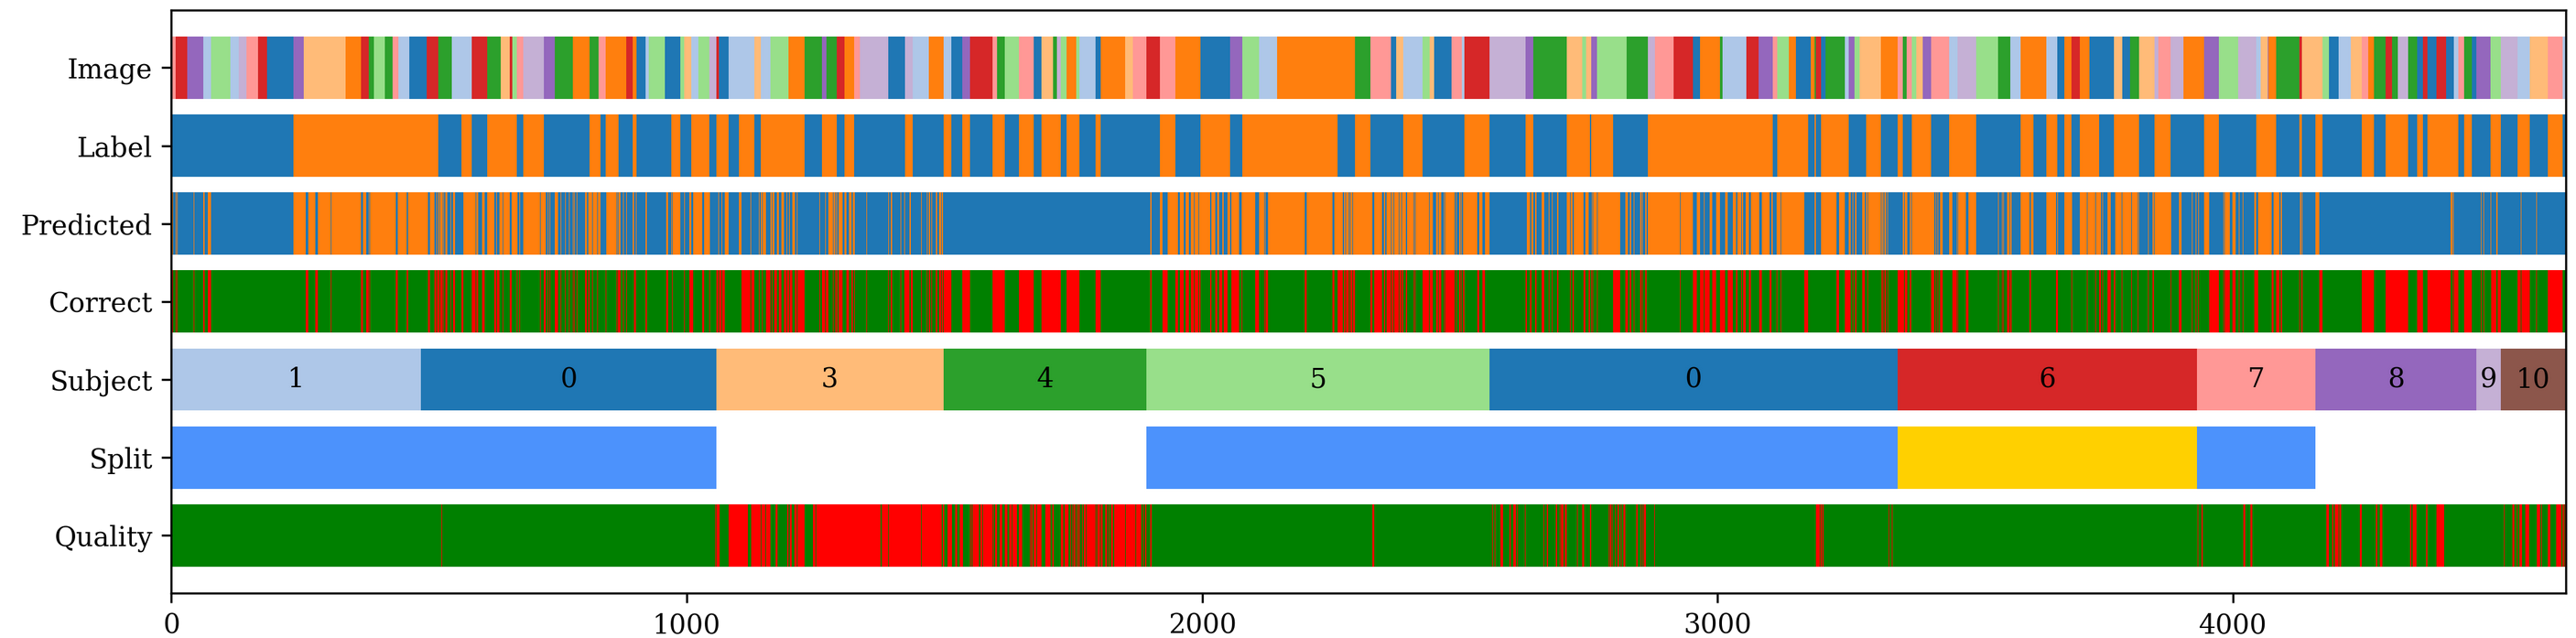
\includegraphics[width=24cm]{img/timebars.png}
                \caption{Visualization of the labeled data with classifications from one fold. Shows the \emph{Image} (stimuli), the \emph{Label} for that stimuli, the \emph{Predicted} class, whether the prediction is \emph{Correct}, the \emph{Subject}, the \emph{Split}/Fold, and our threshold measure for signal \emph{Quality}. The x-axis is the window index, sorted by acquisition time.
                \\
                \\
                It can be seen that (1) subjects \#3 and \#4 have bad signal quality, and have therefore been excluded from the training set. (2) The subjects \#9 and \#10 have also been excluded from training due to issues during data collection. (3) For subject \#1 the stimuli images were not shuffled. (4) Subject \#0 appears twice, as they did two sessions (using unseen stimuli).}\label{fig:timebars}
            \end{figure}
        \end{landscape}

        \begin{comment}
            \begin{figure}[h]
            \centering
            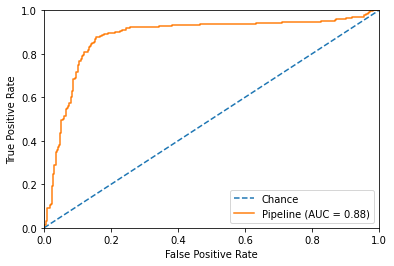
\includegraphics[width=12cm]{img/roccurve.png}
            \caption{Receiver operating characteristic (ROC) curve for subject \#6.}\label{fig:roc}
            \end{figure}
            \change[inline]{Update with higher-res image}
        \end{comment}

    \section{Naturalistic device activity}

        As described in Section~\ref{section:collect-eeg-naturalistic}, we collected approximately \SI{5}{hours} of labeled EEG data using our labels described in Section~\ref{section:collect-usage}.

        Using that data, we trained classifiers for the label pairs:

        \begin{itemize}
                \item Programming / Writing
                \item Programming / Twitter
                \item Twitter / YouTube
        \end{itemize}

        Our results are seen in Table~\ref{table:scores-natural}.

        \begin{table}[h]
            \centering
            \begin{tabular}{llrr}
                \toprule
                Experiment & Score & Support & Hours of data \\
                \midrule
                Programming vs Writing & 0.676 & (1386, 209) & 2.22h \\
                Programming vs Twitter & 0.695 &  (1386, 949) & 3.24h \\
                Twitter vs YouTube & 0.604 & (949, 266) & 1.69h \\
                \bottomrule
            \end{tabular}
            \caption{The scores for each label pairing. The score is the mean balanced accuracy of the StratifiedKFold splits.}\label{table:scores-natural}
        \end{table}

\chapter{Discussion}\label{section:discussion}

We now move on to discussing our results. We will also discuss some threats to the validity, potential applications, ethical considerations, and a brief mention of research initiatives we've contributed to along the way.

As stated earlier in the section ``Aim of the thesis'' (\ref{section:aim}), we set out to answer two research questions:

\paragraph*{RQ1. Can we improve upon previous results in classifying code vs prose comprehension with EEG\@?}

We found that we do improve upon the best classifier performance by Fucci et al.\ in their EEG-only configuration~\cite{fucci_replication_2019}. However, we had to remove certain subjects from our sample, and our sample in general was smaller and more homogenous.\footnote{The reason for this cherry-picked subject selection is due to issues with signal quality and limited data (due to spurious device disconnects).}

Our findings also show that Riemannian methods, as used in this paper, are better at distinguishing between the code and prose tasks than the bandpower-features approach, as used by Fucci et al. Our Riemannian score\footnote{Scores taken from Table~\ref{table:compare-results}} was $0.75$, which is better than both our bandpower-features score of $0.69$, as well as the Fucci et al score of $0.66$. This is in line with our expectations, as Riemannian methods are considered state-of-the-art for many EEG and BCI tasks, unlike bandpower features.

We were not able to outperform the results by Floyd et al.~\cite{floyd_decoding_2017}. This is not surprising given they were using fMRI, which has far superior spatial resolution and can therefore accurately detect elevated activity in specific brain regions over the duration of an epoch. However, our method using EEG has the benefit of high temporal resolution, allowing classification using small amounts of data, enabling near real-time applications.

\paragraph*{RQ2. Can we train an EEG classifier to separate software developers’ device activities?}

We train several classifiers and achieve promising results. We were especially successful in distinguishing work (writing code) from social media (Twitter).

Among the classifiers we train, we found that discerning leisure-activities from each other (such as YouTube vs Twitter) is harder than discerning work from leisure (such as writing code vs Twitter). We also find that EEG is sufficient to not only pick up differences in code vs prose \emph{comprehension} but also in \emph{writing}.

We conclude that our preliminary results indicate that it is possible to discern several different device activities using EEG\@. However, more data from multiple subjects are needed in future work to validate the method and results. 

\section{Threats to validity}\label{section:threats}

    During our work we have considered several potential threats to validity. Some of these arise from our limited and biased dataset, while others are about the task and methodology.

    Starting with our dataset, we collected on mostly right-handed males in their late 20s. This uniform/homogenous sample may lead to less data needed to train a classifier for that particular group, but does not necessarily generalize well to the population at large. Future studies should include a more diverse sample of participants.

    We also had issues during data collection with spurious disconnects from the device, leading to data loss and incomplete experiment runs. This is a threat to the validity of the study due to not all subjects having undergone as many (or the same) trials.

    Among our considerations, one threat to the validity is the stimuli images themselves (seen in Figure~\ref{fig:tasks}). In Floyd et al.~the images used for prose comprehension are in fact more like a code review task, while Fucci et al.~modified the images to test comprehension, instead of ability to judge correctness. We also discovered that subjects found the prose stimuli used by Floyd et al.~confusing, and it would have been preferable to use prose stimuli more like that used by Fucci et al.

    The stimuli images differ on more than just content. Examples of such differences are the background color, the difference in eye saccades while reading (eyes jump around more during the code tasks, where the user may have to jump between the code and the question about it). We have not been able to discard the possibility that the front-heavy electrode placements (with reference electrode at Fpz) lead to much of the signal being from eye saccades. 

    Future research could evaluate this further either by using an eye tracker or by using an EEG device with different placements of both the electrodes and reference electrode.

    %\add[inline]{Investigate threats to validity mentioned by previous authors}

\section{Applications to software engineering}

As we mentioned in the introduction, gaining insight into the brains of developers at work can be used to aid and enhance the productivity of developers in several ways.

Some to assist in development, like helping to identify developer confusion, but other applications could be imagined where a summary of the developers' brain activity during a particular commit (such as if the developer was confused, focused, tired).

%\add[inline]{Include mention and image of mood attached in commit message from Fucci talk?}

Applications of our results include:

\begin{itemize}
    \item Use the confidence in the task prediction as an alternative measurement of focus (not merely measuring that the subject was focused, but what they were focused on). 
    \item Detecting distraction.
    %\item The ability to collect all data needed to train an EEG classifier during normal device use.
\end{itemize}

We also consider our novel idea of `mental churn', a neurally integrated alternative to the measure of code churn, where not only code changes are measured, but also the \emph{attention} a file or piece of code receives as a whole. It can be viewed as quantifying the \emph{cognitive load} of the developer, and attributing it to the current context. This notion of mental churn could also include what response the code elicited in an engineer (confusion, focus, confidence).

\section{Ethical considerations}

    When studying EEG data a range of ethical considerations arise. 

    \begin{itemize}
        \item Could the data be considered personally identifiable information (PII)? 
        \item How privacy sensitive are EEG recordings? Could they contain something the subject would rather keep private? (could have medical implications)
        \item How do we build large public datasets, while preserving participants privacy?
        %\item How can one use EEG in a work environment without unreasonable surveillance of the employee?
    \end{itemize}

    Companies such as Neurosity have taken an approach with their products where all the processing happens on-device, and only aggregates and classifier outputs are sent to the cloud for storage and presentation to the user. This is similar to the approach taken by ActivityWatch for device usage data, where all data is stored locally and never sent to a remote server for processing. 

    We believe this approach is the most privacy-preserving, but it comes at the cost of difficulty in building large datasets, as the data is no longer collected in a central repository under the control of companies or service providers. Therefore, there is a need to bridge the gap between privacy and sharing data.

    Simple solutions to this problem include opt-in to data collection, which is easy to do at scale for companies offering EEG devices. But other efforts include projects such as the NeuroTech Challenge (mentioned in Section~\ref{section:ntcs}).

    There are also more advanced solutions, such as privacy-preserving ML systems. One example of such solutions is \href{https://github.com/OpenMined/PySyft}{PySyft}, which enables private deep learning using federated learning, differential privacy, and encrypted computation (through Multi-Party Computation and Homomorphic Encryption) to work within common deep learning frameworks such as PyTorch and Tensorflow.

\section{Democratization of neuroscience}

    This thesis was made possible due to the efforts of individuals and communities such as NeuroTechX to democratize neuroscience. Indeed, it is the explicit goal of the NeuroTechX eeg-notebooks project to `democratize the neuroscience experiment'. Combined with the rapid cost reduction of research-grade EEG equipment over the last decade it has enabled hobbyists to design and perform high-quality neuroscience experiments. This enables citizen scientists to contribute to data collection, an example of such an effort is the NeuroTech Challenge Series (described in Section~\ref{section:ntcs}).

    As development of BCIs advance and the consumer market for EEG devices grow (as evidenced by new devices being released with a regular cadence by InteraXon and Neurosity) we expect to see more uses and applications of these devices.

    Much of this work was made possible due to the efforts of communities such as NeuroTechX to democratize neuroscience by publishing tools for running experiments. As part of the thesis, we have contributed changes back to some of the tools used (as mentioned in~\Vref{section:aim}).

\subsection{Crowdsourcing data}

    Collecting data is a significant time sink for researchers, and efforts to crowdsource data from the general public are difficult for EEG as it still requires access to the equipment, the knowledge to operate it, as well as considerations like signal quality, electrode placement, and other factors that might invalidate the data.

    Crowdsourcing data comes with new challenges. One of them is that data is now recorded by many different devices, with differences in channel count, sampling rate, electrode placement, and so on, that are difficult to combine in the same dataset. 

    A potential solution to the problem of learning new variations from a small additional sample is to attempt cross-task or cross-subject transfer learning. In such a setup, a model is already trained on a group of subjects, or a similar task, and through a small amount of new data for a particular subject or task, the model can adapt to learn those previously unseen subjects or tasks. This is discussed further in Section~\ref{section:transfer-learning}.

    %\paragraph*{NeuroTech Challenge Series}

    As part of the thesis work I have contributed to the \href{https://neurotech-challenge.com/}{NeuroTech Challenge Series} (NTCS), an effort in crowdsourcing EEG data using the experiments built in \texttt{eeg-notebooks}. The challenge can be performed by anyone with access mobile consumer EEG devices, like those from Muse, OpenBCI, and Neurosity\@. The project is a collaborative effort led by John Griffiths at the University of Toronto, with support from OpenBCI and NeuroTechX.\label{section:ntcs}


\section{Transfer learning}\label{section:transfer-learning}

An important aspect, as highlighted earlier in this thesis, is the ability of a classifier to be able to work on subjects unseen in training. Some BCI systems employ a calibration phase to achieve greater performance, but this can be time-consuming and straining for the user.

To minimize this need for calibration is a stated research goal in Khazem et al.~\cite{khazem_minimizing_2021}, which presents what is called Riemannian Transfer Learning. They build on Riemannian geometry used in state-of-the-art classifiers, and develop a variation of MDM (explained in Section~\ref{section:riemannian-theory}) called \emph{Minimum Distance to Weighted Mean} (MDWM). The method takes a parameter $\lambda$ (where $0 \leq \lambda \leq 1$) that controls how much the algorithm should rely on the class centroids learned from past subjects versus the calibration data from a new subject. This is useful in online learning contexts, where the parameter can initially start at $0$ and then be incrementally adjusted towards $1$. The researchers found $\lambda = 0.7$ to be a reasonable value for many tasks. 

The researchers also considered using weights for each source subject as done by Kalunga et al.~\cite{kalunga_transfer_2018}, which could be used to adjust for subject similarity.

We investigated this avenue of inquiry to potentially minimize the amount of data collection needed, but in the end did not have the time to implement it.

\chapter{Conclusions}

Our results successfully replicate previous research, showing that it is possible to distinguish between reading code and prose using EEG, and improves upon the state of the art in this regard by achieving a roughly $\sim$75\% balanced accuracy (using LORO cross-validation). However, the reader should note limitations of our study in Section~\ref{section:threats}.

Furthermore, our naturalistic experiments indicate it is possible to distinguish many other device activities from each other using consumer-grade EEG devices. Among these some data seems to suggest that EEG is sufficient to not only pick up differences in code vs prose \emph{comprehension} but also in \emph{writing}.

\section{Future work}

Future work could integrate the code vs prose task into \texttt{moabb} to make it easier to replicate the results and evaluate new methods. As mentioned, the study would also benefit from more data collection, possibly through the NeuroTech Challenge Series (mentioned in Section~\ref{section:ntcs}).

As mentioned in the method, this study uses prose \emph{review} images from Floyd et al., as opposed to the prose \emph{comprehension} images (in Italian) used by Fucci et al. Ideally, one should create an English prose comprehension set of stimuli images, similar to the ones used by Fucci.

We also encourage researchers to experiment with our naturalistic device use classification. In particular, future work could extend our method by collecting data on more subjects and activities.


% Pagebreak after glossary
\vfill
\pagebreak

% References
%\bibbysegment{}
\printbibliography[category=cited]

% Further reading (uncited)
\nocite{*}
\defbibenvironment{bibnonum}
  {\list{}
     {\setlength{\leftmargin}{\bibhang}%
      \setlength{\itemindent}{-\leftmargin}%
      \setlength{\itemsep}{\bibitemsep}%
      \setlength{\parsep}{\bibparsep}}
  }
  {\endlist}
  {\item}
\printbibliography[notcategory=cited, env=bibnonum, heading=notcited]

\pagebreak

% Glossary
\printglossary
\printglossary[title=Acronyms, type=\acronymtype, toctitle=Glossary]

\end{refsection}
\end{document}
